\documentclass[a4paper,12pt,twoside]{memoir}

% Castellano
\usepackage[spanish,es-tabla]{babel}
\selectlanguage{spanish}
\usepackage[utf8]{inputenc}
\usepackage[T1]{fontenc}
\usepackage{lmodern} % scalable font
\usepackage{microtype}
\usepackage{placeins}

\RequirePackage{booktabs}
\RequirePackage[table]{xcolor}
\RequirePackage{xtab}
\RequirePackage{multirow}

% Links
\PassOptionsToPackage{hyphens}{url}\usepackage[colorlinks]{hyperref}
\hypersetup{
	allcolors = {blue}
}

% Ecuaciones
\usepackage{amsmath}

% Rotar imagenes
\usepackage{rotating}

% Rutas de fichero / paquete
\newcommand{\ruta}[1]{{\sffamily #1}}

% Párrafos
\nonzeroparskip

% Huérfanas y viudas
\widowpenalty100000
\clubpenalty100000

% Evitar solapes en el header
\nouppercaseheads

% Imagenes
\usepackage{graphicx}
\newcommand{\imagen}[2]{
	\begin{figure}[!h]
		\centering
		\includegraphics[width=0.9\textwidth]{#1}
		\caption{#2}\label{fig:#1}
	\end{figure}
	\FloatBarrier
}

\newcommand{\imagenflotante}[2]{
	\begin{figure}%[!h]
		\centering
		\includegraphics[width=0.9\textwidth]{#1}
		\caption{#2}\label{fig:#1}
	\end{figure}
}



% El comando \figura nos permite insertar figuras comodamente, y utilizando
% siempre el mismo formato. Los parametros son:
% 1 -> Porcentaje del ancho de página que ocupará la figura (de 0 a 1)
% 2 --> Fichero de la imagen
% 3 --> Texto a pie de imagen
% 4 --> Etiqueta (label) para referencias
% 5 --> Opciones que queramos pasarle al \includegraphics
% 6 --> Opciones de posicionamiento a pasarle a \begin{figure}
\newcommand{\figuraConPosicion}[6]{%
  \setlength{\anchoFloat}{#1\textwidth}%
  \addtolength{\anchoFloat}{-4\fboxsep}%
  \setlength{\anchoFigura}{\anchoFloat}%
  \begin{figure}[#6]
    \begin{center}%
      \Ovalbox{%
        \begin{minipage}{\anchoFloat}%
          \begin{center}%
            \includegraphics[width=\anchoFigura,#5]{#2}%
            \caption{#3}%
            \label{#4}%
          \end{center}%
        \end{minipage}
      }%
    \end{center}%
  \end{figure}%
}

%
% Comando para incluir imágenes en formato apaisado (sin marco).
\newcommand{\figuraApaisadaSinMarco}[5]{%
  \begin{figure}%
    \begin{center}%
    \includegraphics[angle=90,height=#1\textheight,#5]{#2}%
    \caption{#3}%
    \label{#4}%
    \end{center}%
  \end{figure}%
}
% Para las tablas
\newcommand{\otoprule}{\midrule [\heavyrulewidth]}
%
% Nuevo comando para tablas pequeñas (menos de una página).
\newcommand{\tablaSmall}[5]{%
 \begin{table}
  \begin{center}
   \rowcolors {2}{gray!35}{}
   \begin{tabular}{#2}
    \toprule
    #4
    \otoprule
    #5
    \bottomrule
   \end{tabular}
   \caption{#1}
   \label{tabla:#3}
  \end{center}
 \end{table}
}

%
%Para el float H de tablaSmallSinColores
\usepackage{float}

%
% Nuevo comando para tablas pequeñas (menos de una página).
\newcommand{\tablaSmallSinColores}[5]{%
 \begin{table}[H]
  \begin{center}
   \begin{tabular}{#2}
    \toprule
    #4
    \otoprule
    #5
    \bottomrule
   \end{tabular}
   \caption{#1}
   \label{tabla:#3}
  \end{center}
 \end{table}
}

\newcommand{\tablaApaisadaSmall}[5]{%
\begin{landscape}
  \begin{table}
   \begin{center}
    \rowcolors {2}{gray!35}{}
    \begin{tabular}{#2}
     \toprule
     #4
     \otoprule
     #5
     \bottomrule
    \end{tabular}
    \caption{#1}
    \label{tabla:#3}
   \end{center}
  \end{table}
\end{landscape}
}

%
% Nuevo comando para tablas grandes con cabecera y filas alternas coloreadas en gris.
\newcommand{\tabla}[6]{%
  \begin{center}
    \tablefirsthead{
      \toprule
      #5
      \otoprule
    }
    \tablehead{
      \multicolumn{#3}{l}{\small\sl continúa desde la página anterior}\\
      \toprule
      #5
      \otoprule
    }
    \tabletail{
      \hline
      \multicolumn{#3}{r}{\small\sl continúa en la página siguiente}\\
    }
    \tablelasttail{
      \hline
    }
    \bottomcaption{#1}
    \rowcolors {2}{gray!35}{}
    \begin{xtabular}{#2}
      #6
      \bottomrule
    \end{xtabular}
    \label{tabla:#4}
  \end{center}
}

%
% Nuevo comando para tablas grandes con cabecera.
\newcommand{\tablaSinColores}[6]{%
  \begin{center}
    \tablefirsthead{
      \toprule
      #5
      \otoprule
    }
    \tablehead{
      \multicolumn{#3}{l}{\small\sl continúa desde la página anterior}\\
      \toprule
      #5
      \otoprule
    }
    \tabletail{
      \hline
      \multicolumn{#3}{r}{\small\sl continúa en la página siguiente}\\
    }
    \tablelasttail{
      \hline
    }
    \bottomcaption{#1}
    \begin{xtabular}{#2}
      #6
      \bottomrule
    \end{xtabular}
    \label{tabla:#4}
  \end{center}
}

%
% Nuevo comando para tablas grandes sin cabecera.
\newcommand{\tablaSinCabecera}[5]{%
  \begin{center}
    \tablefirsthead{
      \toprule
    }
    \tablehead{
      \multicolumn{#3}{l}{\small\sl continúa desde la página anterior}\\
      \hline
    }
    \tabletail{
      \hline
      \multicolumn{#3}{r}{\small\sl continúa en la página siguiente}\\
    }
    \tablelasttail{
      \hline
    }
    \bottomcaption{#1}
  \begin{xtabular}{#2}
    #5
   \bottomrule
  \end{xtabular}
  \label{tabla:#4}
  \end{center}
}



\definecolor{cgoLight}{HTML}{EEEEEE}
\definecolor{cgoExtralight}{HTML}{FFFFFF}

%
% Nuevo comando para tablas grandes sin cabecera.
\newcommand{\tablaSinCabeceraConBandas}[5]{%
  \begin{center}
    \tablefirsthead{
      \toprule
    }
    \tablehead{
      \multicolumn{#3}{l}{\small\sl continúa desde la página anterior}\\
      \hline
    }
    \tabletail{
      \hline
      \multicolumn{#3}{r}{\small\sl continúa en la página siguiente}\\
    }
    \tablelasttail{
      \hline
    }
    \bottomcaption{#1}
    \rowcolors[]{1}{cgoExtralight}{cgoLight}

  \begin{xtabular}{#2}
    #5
   \bottomrule
  \end{xtabular}
  \label{tabla:#4}
  \end{center}
}




\graphicspath{ {./img/} }

% Capítulos
\chapterstyle{bianchi}
\newcommand{\capitulo}[2]{
	\setcounter{chapter}{#1}
	\setcounter{section}{0}
	\chapter*{#2}
	\addcontentsline{toc}{chapter}{#2}
	\markboth{#2}{#2}
}

% Apéndices
\renewcommand{\appendixname}{Apéndice}
\renewcommand*\cftappendixname{\appendixname}

\newcommand{\apendice}[1]{
	%\renewcommand{\thechapter}{A}
	\chapter{#1}
}

\renewcommand*\cftappendixname{\appendixname\ }

% Formato de portada
\makeatletter
\usepackage{xcolor}
\newcommand{\tutor}[1]{\def\@tutor{#1}}
\newcommand{\course}[1]{\def\@course{#1}}
\definecolor{cpardoBox}{HTML}{E6E6FF}
\def\maketitle{
  \null
  \thispagestyle{empty}
  % Cabecera ----------------
\noindent
\includegraphics[width=\textwidth]{cabecera}\vspace{1cm}%
  \vfill
  % Título proyecto y escudo informática ----------------
  \colorbox{cpardoBox}{%
    \begin{minipage}{.8\textwidth}
      \vspace{.5cm}\Large
      \begin{center}
      \textbf{TFG del Grado en Ingeniería Informática}\vspace{.6cm}\\
      \textbf{\LARGE\@title{}}
      \end{center}
      \vspace{.2cm}
    \end{minipage}

  }%
  \hfill\begin{minipage}{.20\textwidth}
    
\includegraphics[width=\textwidth]{escudoInfor}
  \end{minipage}
  \vfill
  % Datos de alumno, curso y tutores ------------------
  \begin{center}%
  {%
    \noindent\LARGE
    Presentado por \@author{}\\ 
    en Universidad de Burgos --- \@date{}\\
    Tutor: \@tutor{}\\
  }%
  \end{center}%
  \null
  \cleardoublepage
  }
\makeatother

\newcommand{\nombre}{Pablo Fernández Bravo} %%% cambio de comando

% Datos de portada
\title{GTM - Plataforma de experimentación de Text Mining sobre repositorios de GitHub \\Documentación Técnica}
\author{\nombre}
\tutor{Dr. Carlos López Nozal y \\ D. Jesús María Alonso Abad}
\date{\today}

%in the preamble
%--------------------------------
  \usepackage[
    backend=biber,
    style=numeric,
  ]{biblatex}
  \usepackage{csquotes}
  \usepackage{multirow}
  \usepackage{tablefootnote}
  \usepackage{numprint}

 \addbibresource{bibliografiaAnexos.bib}
%--------------------------------

\begin{document}

\maketitle



\cleardoublepage



%%%%%%%%%%%%%%%%%%%%%%%%%%%%%%%%%%%%%%%%%%%%%%%%%%%%%%%%%%%%%%%%%%%%%%%%%%%%%%%%%%%%%%%%



\frontmatter


\clearpage

% Indices
\tableofcontents

\clearpage

\listoffigures

\clearpage

\listoftables

\clearpage

\mainmatter

\appendix

\apendice{Plan de Proyecto Software}

\section{Introducción}

El plan de proyecto presenta al lector un estudio del proceso organizativo y de gestión seguido a lo largo del desarrollo del proyecto con el propósito de cumplir con los objetivos propuestos dentro de los plazos establecidos. 

En los siguientes apartados se detallan los aspectos relativos a la distribución de las tareas, el estudio de los gastos asumidos durante la realización del proyecto y los aspectos legales relativos a la propiedad intelectual de los ficheros del proyecto, incluyendo su documentación y dependencias.


\section{Planificación temporal}

La planificación de temporal de los objetivos del proyecto se ha realizado siguiendo las recomendaciones de la metodología ágil SCRUM. La base de esta metodología consta de la realización periódica de reuniones que permitan mantener un control sobre el progreso en las tareas propuestas para cada Sprint.

Estas reuniones coincidirían con la finalización de cada Sprint y constarían de dos partes. Una primera parte se centraría en la finalización del Sprint, donde se trataría de presentar los avances realizados en los objetivos, se presentarían los problemas encontrados y las soluciones propuestas para su resolución. En la segunda parte se propondrían las tareas y planificación del siguiente Sprint a partir de la retroalimentación obtenida por los tutores del proyecto.

\subsection{Sprint 1: Toma de Contacto}

El sprint inicial tuvo lugar tras la aprobación del proyecto. Durante la reunión inicial se establecieron algunos de los objetivos generales que se perseguían con su realización. Partiendo de cero se propuso llevar a cabo el desarrollo mediante el uso de Python debido a que se disponía de un mayor conocimiento en dicho lenguaje. 

Uno de los objetivos principales del proyecto sería trabajar con datos extraídos de la plataforma GitHub. Durante este sprint se decidió realizar un prototipo que permitiese llevar a cabo la descarga de información de repositorios públicos mediante el uso de la API REST de GitHub. Para ello se localizaron módulos de Python que simplificaban el proceso de realización de llamadas a GitHub y el tratamiento de la información recibida. Se realizó un estudio del funcionamiento de las diversas alternativas hasta seleccionar el paquete más se adaptase a las necesidades del proyecto de acuerdo con la calidad de su implementación y la disponibilidad de una documentación adecuada.

\subsubsection{Listado de tareas}

\begin{itemize} \setlength\itemsep{0.2em}
    \item \href{https://github.com/MrpYA45/github-text-mining-tfg/issues/1}{Investigar sobre la conexión con GitHub} [3h].
    \item \href{https://github.com/MrpYA45/github-text-mining-tfg/issues/3}{Prototipar la descarga de issues mediante PyGithub} [3h].
    \item \href{https://github.com/MrpYA45/github-text-mining-tfg/issues/4}{Testear las limitaciones de la API de GitHub} [2h].
\end{itemize}

\subsection{Sprint 2: Primera iteración de la extracción y almacenamiento de la información.}

El segundo sprint del proyecto contempla la planificación de la arquitectura del proyecto con la finalidad de diseñar una arquitectura de microservicios de acuerdo con los objetivos del proyecto. Para ello, se realizó un estudio de los servicios requeridos para cumplir con las funcionalidades previstas de la aplicación y la forma de mantener la comunicación entre ellos.

Una vez se tomaron estas decisiones se dio comienzo al diseño e implementación de la estructura de la base de datos a través del mapeo de objetos relacionales mediante el uso del paquete SQLAlchemy. Este paquete actuaría como dependencia del servicio principal en cada uno de los servicios, permitiendo su acceso al contenido de la base de datos.

\subsubsection{Listado de tareas}

\begin{itemize} \setlength\itemsep{0.2em}
    \item \href{https://github.com/MrpYA45/github-text-mining-tfg/issues/6}{Realizar el cambio de biblioteca que maneja la conexión con GitHub} [2h].
    \item \href{https://github.com/MrpYA45/github-text-mining-tfg/issues/8}{Crear un prototipo para la base de datos} [10h].
    \item \href{https://github.com/MrpYA45/github-text-mining-tfg/issues/7}{Crear un administrador para la descarga de los repositorios} [10h].
    \item \href{https://github.com/MrpYA45/github-text-mining-tfg/issues/9}{Tratamiento de las excepciones de la base de datos y de la extracción de GitHub} [3h].
\end{itemize}

\subsection{Sprint 3: Primera iteración de la API REST y concurrencia.}

En este tercer sprint se realizó la primera implementación del servicio de API REST junto a un pequeño front-end que permitiría realizar una serie de comprobaciones básicas. También se desarrollarían una serie de scripts que permitirían automatizar la detección y comprobación de errores de tipado por medio de las GitHub Actions. De manera paralela se realizó un estudio de las posibilidades de implementar la concurrencia en la descarga de los repositorios.

\subsubsection{Listado de tareas}

\begin{itemize} \setlength\itemsep{0.2em}
    \item \href{https://github.com/MrpYA45/github-text-mining-tfg/issues/11}{Estudiar la aplicación de concurrencia en Python} [6h].
    \item \href{https://github.com/MrpYA45/github-text-mining-tfg/issues/13}{Implementar las Acciones de GitHub para la comprobación de tipado y estilo} [2h].
    \item \href{https://github.com/MrpYA45/github-text-mining-tfg/issues/14}{Primera implementación básica de Flask } [4h].

\end{itemize}

\subsection{Sprint 4: Microservicios y Flask}

En este cuarto sprint se diseño una configuración de Docker que permitiría el despliegue de la aplicación en un contenedor propio. Para adaptar la aplicación a Docker se realizó una reorganización de los paquetes y se diseñaron una serie de scripts que permitirían lanzar los servicios automáticamente al arrancar los contenedores.

\subsubsection{Listado de tareas}

\begin{itemize} \setlength\itemsep{0.2em}
    \item \href{https://github.com/MrpYA45/github-text-mining-tfg/issues/10}{Documentación del código de la capa de datos y la capa lógica} [4h].
    \item \href{https://github.com/MrpYA45/github-text-mining-tfg/issues/2}{Explorar la organización de la arquitectura de microservicios } [6h].
    \item \href{https://github.com/MrpYA45/github-text-mining-tfg/issues/17}{Creación de scripts bash que permitan la instalación y ejecución de la aplicación} [4h].
    \item \href{https://github.com/MrpYA45/github-text-mining-tfg/issues/16}{Rediseño del software - Diseño evolutivo} [5h].
    \item \href{https://github.com/MrpYA45/github-text-mining-tfg/issues/15}{Implementación de Docker para el despliegue de la aplicación. } [3h].

\end{itemize}

\subsection{Sprint 5: Primera iteración del servicio de procesamiento.}

Este quinto sprint se logró implementar la primera aproximación del servicio de procesamiento incluyendo el modelo de clasificación Zero-Shot. También se actualizó el servicio de extracción para contemplar la recogida de las etiquetas del repositorio.

\subsubsection{Listado de tareas}

\begin{itemize} \setlength\itemsep{0.2em}
    \item \href{https://github.com/MrpYA45/github-text-mining-tfg/issues/21}{Mejora y adición de métodos para poder introducir el procesamiento } [6h].
    \item \href{https://github.com/MrpYA45/github-text-mining-tfg/issues/22}{Recoger los datos de las etiquetas de los repositorios} [4h].
    \item \href{https://github.com/MrpYA45/github-text-mining-tfg/issues/23}{Implementar modelo NLP Zero Shot Classifier } [8h].

\end{itemize}
 
\subsection{Sprint 6: Segunda iteración del servicio de procesamiento.}

En este sexto sprint adoptó el lanzamiento de los diferentes servicios que componen la aplicación en contenedores separados a través de docker-compose, de esta manera los servicios podrían mantenerse aislados los unos de los otros.

\subsubsection{Listado de tareas}

\begin{itemize} \setlength\itemsep{0.2em}
    \item \href{https://github.com/MrpYA45/github-text-mining-tfg/issues/25}{Separación de módulos en diferentes contenedores mediante docker-compose} [12h].
    \item \href{https://github.com/MrpYA45/github-text-mining-tfg/issues/28}{Añadir la detección y descarga automática de modelos cuando no se posean} [4h].
\end{itemize}

\subsection{Sprint 7: Actualización de la base de datos e introducción de los ficheros de configuración.}

En este séptimo sprint se decidió reemplazar el uso SQLite como gestor de base de datos por MariaDB debido a los problemas de concurrencia derivados del aislamiento de los servicios en distintos contenedores. En el servicio de procesamiento se implementó un sistema encargado de descargar los modelos desde Hugging Face de manera que mantuviesen de forma local en el equipo.

\subsubsection{Listado de tareas}

\begin{itemize} \setlength\itemsep{0.2em}
    \item \href{https://github.com/MrpYA45/github-text-mining-tfg/issues/27}{Crear/Actualizar el fichero de configuración por módulo} [4h].
    \item \href{https://github.com/MrpYA45/github-text-mining-tfg/issues/26}{Cambiar la base de datos de SQLite a MariaDB } [8h].
\end{itemize}

\subsection{Sprint 8: Tercera iteración del servicio de procesamiento.}

En este octavo sprint se centra en la implementación de estrategias que permitan someter a la información extraída a un preprocesado donde se eliminen las impurezas de los datos con el objetivo de mejorar los resultados de los modelos.

En adición a estas estrategias, se tomó como referencia los algoritmos de división de textos y optimización del contexto implementados en el proyecto <<JIZT>> buscando obtener mejores resultados ante entradas de los modelos que superasen las limitaciones relativas al tamaño de las entradas de los modelos.

\subsubsection{Listado de tareas}

\begin{itemize} \setlength\itemsep{0.2em}
    \item \href{https://github.com/MrpYA45/github-text-mining-tfg/issues/29}{Creación de utilidades para el tratamiento de la información extraída} [6h].
    \item \href{https://github.com/MrpYA45/github-text-mining-tfg/issues/30}{Implementación de algoritmos de sección y balanceo de textos} [15h].
    \item \href{https://github.com/MrpYA45/github-text-mining-tfg/issues/34}{Almacenamiento de los resultados de los modelos} [15h].
    \item \href{https://github.com/MrpYA45/github-text-mining-tfg/issues/31}{Implementación de las tareas de resumen} [20h].
    \item \href{https://github.com/MrpYA45/github-text-mining-tfg/issues/32}{Implementación de las tareas de análisis de sentimientos} [20h].
    \item \href{https://github.com/MrpYA45/github-text-mining-tfg/issues/33}{Ajuste de la extracción para el uso de las nuevas utilidades de preprocesamiento} [10h].
    \item \href{https://github.com/MrpYA45/github-text-mining-tfg/issues/5}{Explorar modelos pre-entrenado para resolver tareas de NLP } [8h].
\end{itemize}

\subsection{Sprint 9: Segunda iteración de la API REST y primera iteración de la aplicación web.}

En este noveno sprint se eliminan las vistas de la aplicación del servicio de API REST, implementando numerosos endpoints en su lugar. A raíz de la anterior decisión comienza el desarrollo de una aplicación web basada en el framework React con el objetivo de que los usuarios sean capaces de interactuar con la API REST a través de una interfaz gráfica.

\subsubsection{Listado de tareas}

\begin{itemize} \setlength\itemsep{0.2em}
    \item \href{https://github.com/MrpYA45/github-text-mining-tfg/issues/36}{Investigate about React framework } [15h].
    \item \href{https://github.com/MrpYA45/github-text-mining-tfg/issues/35}{Bug fixing and improvements needed at gtmprocessing service. } [15h].
    \item \href{https://github.com/MrpYA45/github-text-mining-tfg/issues/20}{Implementar mejores respuestas de la API REST} [10h].
    \item \href{https://github.com/MrpYA45/github-text-mining-tfg/issues/19}{Mover las vistas de la aplicación al front-end} [20h].
\end{itemize}

\subsection{Sprint 10: Segunda iteración de la aplicación web y realización de pruebas sobre la API REST.}

En este décimo sprint se continua con el desarrollo de la aplicación web, diseñando e implementando los formularios que permitirán a los usuarios el lanzamiento de los experimentos. De manera paralela al desarrollo se comienza a generar la documentación del proyecto (memoria y anexos).

\subsubsection{Listado de tareas}

\begin{itemize} \setlength\itemsep{0.2em}
    \item \href{https://github.com/MrpYA45/github-text-mining-tfg/issues/37}{Realizar pruebas sobre la API REST a través de Postman } [4h].
    \item \href{https://github.com/MrpYA45/github-text-mining-tfg/issues/38}{Implementar los formularios que permitan lanzar los experimentos contra la información extraída de los repositorios } [8h].
\end{itemize}

\subsection{Sprint 11: Tercera iteración de la aplicación web y corrección de errores.}

En este undécimo sprint se realizan pruebas sobre la estabilidad sobre la aplicación y se corrigen los error detectados. La aplicación web recibe un cambio de diseño y se finalizan los componentes encargados de mostrar los resultados de los experimentos.

\subsubsection{Listado de tareas}

\begin{itemize} \setlength\itemsep{0.2em}
    \item \href{https://github.com/MrpYA45/github-text-mining-tfg/issues/40}{Error at gtmextraction module when Repositories or Issues don't have a description} [4h].
    \item \href{https://github.com/MrpYA45/github-text-mining-tfg/issues/41}{Los caracteres Unicode son eliminados dando lugar a textos ilegibles} [1h].
    \item \href{https://github.com/MrpYA45/github-text-mining-tfg/issues/42}{Realización de pruebas sobre la aplicación con una serie de repositorios de diferente naturaleza} [4h].
\end{itemize}

\subsection{Sprint 12: Redacción de los anexos e implementación de correcciones de errores varios.}

Este último sprint se realizan las últimas pruebas sobre el comportamiento de la aplicación en diferentes sistemas operativos. Se aplican las correcciones propuestas sobre la documentación, se generan los anexos y se prepara el proyecto para su entrega.

\subsection{Evaluación del desarrollo}

La evaluación del desarrollo tiene como objetivo presentar un análisis de la distribución del trabajo de acuerdo con los objetivos generales del proyecto. El empleo de la metodología ágil \textbf{SCRUM} ha permitido desarrollar el siguiente diagrama burn-down a través del cual visualizar los plazos esperados para el cumplimiento de las tareas propuestas en cada etapa del desarrollo (véase \autoref{fig:general_burndown_chart}.

\begin{figure}[!ht]
	\centering
    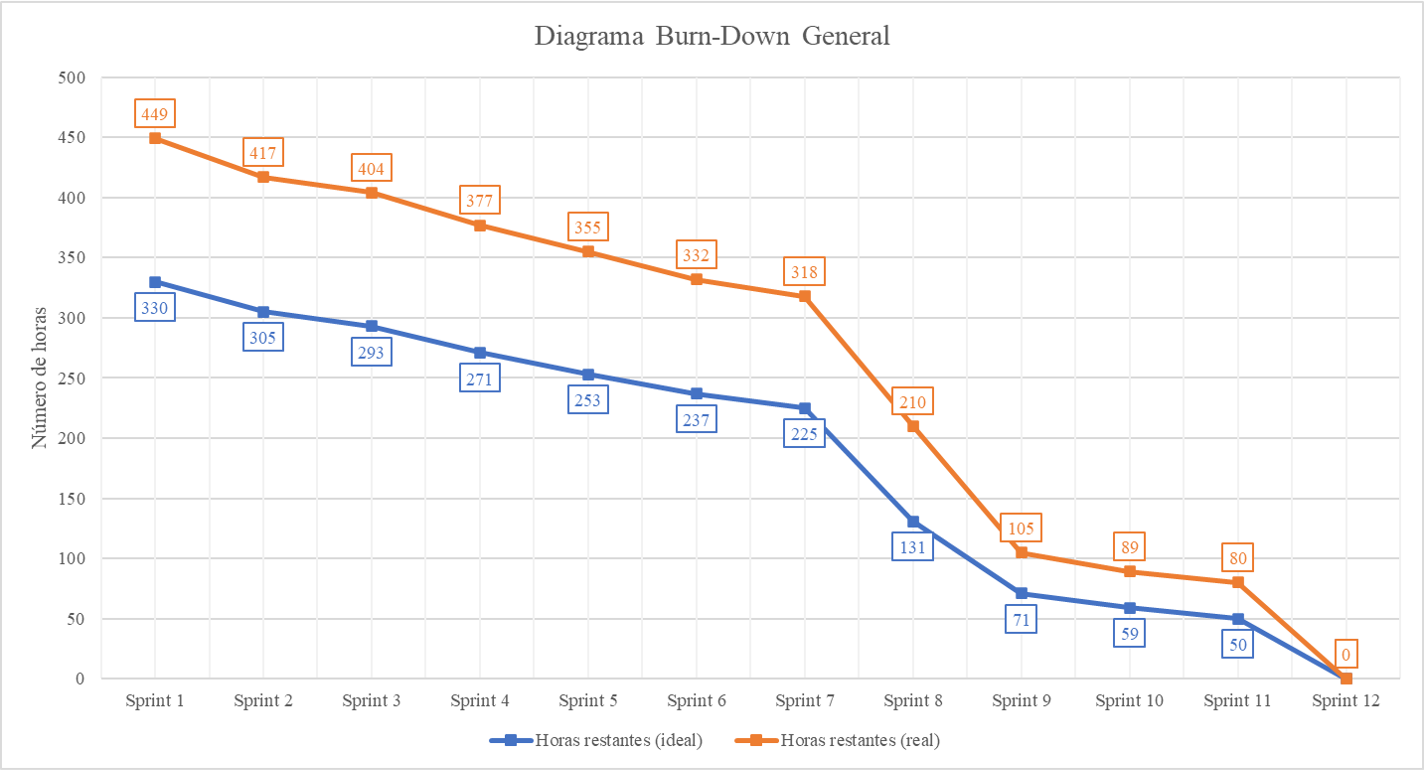
\includegraphics[width=\textwidth]{img/general_burndown_chartpng.png}
	\caption{Diagrama burn-down a nivel de proyecto.}
	\label{fig:general_burndown_chart}
\end{figure}

A la vista de los datos reflejados por el gráfico, se puede observa como a lo largo del proyecto se ha realizado una sobreestimación del esfuerzo requerido para el cumplimiento de las actividades definidas en cada Sprint.

\section{Estudio de viabilidad}

\subsection{Viabilidad económica}

El siguiente apartado tiene como finalidad determinar la viabilidad económica del proyecto, analizando los gastos de inversión necesarios para su desarrollo. En los siguientes secciones se proporciona el desglose de los gastos de personal, gastos hardware y gastos generales requeridos para el desarrollo del proyecto.

\subsubsection{Gastos de personal}

Los gastos de personal representan los gastos que supone contratar al personal requerido para la realización del proyecto. En el caso de nuestro proyecto estos cálculos se realizan considerando que el proyecto ha sido realizado por un único \textbf{programador junior recién egresado}.

El sueldo promedio de un programador junior en España es de \textbf{\numprint{20000} euros brutos anuales} de acuerdo con la información obtenida del portal de la \textbf{Universidad Europea} \cite{ve:salario_ingeniero_informatico}. Realizaremos la estimación de los gastos que supondría mantener a dicho programador a media jornada durante un periodo de 6 meses. En la siguiente tabla se presenta el desglose de los gastos que supondría su contratación.

\tablaSmallSinColores{Desglose de los gastos de personal del proyecto (6 meses)}{l r r}{gastosdepersonal}
{ \multicolumn{1}{l}{\centering\textbf{Concepto}} & \multicolumn{1}{p{2.5cm}}{\raggedleft\textbf{Importe mensual}} & \multicolumn{1}{p{2.5cm}}{\raggedleft\textbf{Importe semestral}} \\}{ 
    \emph{Salario bruto mensual (media jornada)}  & \numprint{833,33} €  & \numprint{5000,00} € \\
    \emph{Contingencias comunes (23,60\%)}        & \numprint{196,67} €  & \numprint{1180,00} € \\
    \emph{Tipo general de desempleo (5,50\%)}     & \numprint{48,83} €   & \numprint{275,00} € \\
    \emph{Fondo de Garantía Salarial (0,20\%)}    & \numprint{1,67} €    & \numprint{10,00} € \\
    \emph{Formación Profesional (0,70\%)}         & \numprint{5,83} €    & \numprint{35,00} € \\ 
    \bottomrule
    \textbf{TOTAL}                                & \numprint{1083,33} € & \numprint{6500,00} € \\
}

\subsubsection{Gastos hardware}

Los gastos hardware se refieren a aquellos dispositivos sobre los que se ha realizado una inversión para cumplir con las necesidades del proyecto. Este tipo de materiales gozan de un periodo de vida útil para el cual se realizan los siguientes cálculos de amortización siguiendo las directrices de los coeficientes de amortización descritos por la Agencia Tributaria \cite{ve:agencia-tributaria-2021}. Se consideran unos costes de amortización por un periodo de \textbf{un año} debido a que el cálculo de este valor se realiza de manera anual.

\tablaSmallSinColores{Desglose gastos hardware del proyecto (Anual)}{l r r}{gastoshardware}
{ \multicolumn{1}{l}{\centering\textbf{Concepto}} & \multicolumn{1}{p{2.5cm}}{\raggedleft\textbf{Importe}} & \multicolumn{1}{p{2.5cm}}{\raggedleft\textbf{Amortización}} \\}{ 
    \emph{Equipo portátil} & \numprint{1000,00} € & \numprint{100,00} € \\
    \emph{Monitor 24''}    & \numprint{150,00} €  & \numprint{15,00} € \\
    \emph{Ratón}           & \numprint{25,00} €   & \numprint{2,50} € \\
    \bottomrule
    \textbf{TOTAL}         & \numprint{1175,00} € & \numprint{117,00} € \\
}

\subsubsection{Gastos generales}

Los gastos generales son aquellos gastos adicionales necesarios para poder llevar a cabo el desarrollo de proyecto. Entre la variedad de supuestos en los que podemos encontrar este tipo de gastos estableceremos una distinción entre aquellos gastos puntuales en materiales específicos requeridos en momentos puntuales, y aquellos gastos de carácter periódico que clasificaremos como gastos de actividad.

En el siguiente desglose se pueden apreciar los gastos material aproximados para cumplir con los requisitos de la entrega de proyecto.

\tablaSmallSinColores{Desglose gastos generales de material del proyecto}{l r}{gastosmaterial}
{ \multicolumn{1}{l}{\centering\textbf{Concepto}} & \multicolumn{1}{p{2.5cm}}{\raggedleft\textbf{Importe}} \\}{
    \emph{Impresión Memoria} & \numprint{30,00} € \\
    \emph{USB 32GB x3}       & \numprint{15,00} € \\
    \bottomrule
    \textbf{TOTAL}           & \numprint{45,00} € \\
}

A continuación, se presenta el desglose de los gastos de actividad surgidos de la necesidad de proporcionar al desarrollador los servicios necesarios para poder cumplir con sus obligaciones durante el desarrollo del proyecto.

\tablaSmallSinColores{Desglose de los gastos generales de actividad del proyecto}{l r r}{gastosactividad}
{ \multicolumn{1}{l}{\centering\textbf{Concepto}} & \multicolumn{1}{p{2.5cm}}{\raggedleft\textbf{Importe mensual}} & \multicolumn{1}{p{2.5cm}}{\raggedleft\textbf{Importe semestral}} \\}{ 
    \emph{Consumo eléctrico}   & \numprint{40,00} €   & \numprint{240,00} € \\
    \emph{Cuota internet}      & \numprint{55,00} €   & \numprint{330,00} € \\
    \emph{Alquiler oficina}    & \numprint{350,00} €  & \numprint{2100,00} € \\
    \emph{Material de oficina} & \numprint{10,00} €   & \numprint{60,00} € \\
    \bottomrule
    \textbf{TOTAL}             & \numprint{455,00} € & \numprint{2730,00} € \\
}

\subsection{Viabilidad legal}

El siguiente apartado tiene como finalidad presentar los aspectos legales del proyecto en referencia a las licencias de uso y distribución de aquellos componentes que conforman el código fuente de la aplicación, así como los relativos a las dependencias y materiales utilizados durante el desarrollo del proyecto.

\subsubsection{Proyecto y Documentación}

El proyecto y su documentación se distribuyen bajo la \textbf{GNU General Public License v3.0} \cite{vl:gplv3} en cumplimiento con las restricciones de uso de aquellos complementos de terceros implicados en el desarrollo y requeridos por la aplicación para su correcto funcionamiento.

La elección de esta licencia de \emph{software libre} responde a la concepción personal de devolver a la comunidad de desarrolladores aquellos conocimientos adquiridos durante su desarrollo. Gracias a los aportes de aquellos desarrolladores que previamente decidieron compartir sus aportes el proyecto ha podido cumplir con los objetivos propuestos.

Las características principales de la licencia \textbf{GNU GPLv3} proporcionan a los futuros interesados en el trabajar con proyecto la capacidad de modificar, distribuir, y utilizar el código tanto de manera comercial, privada o a través de patentes siempre y cuando se incluyan junto con su aplicación el código fuente de este. A su vez, esta licencia exime al creador de ofrecer garantías y responsabilidades sobre el correcto funcionamiento o la aparición de futuros problemas sobre el producto (véase \autoref{fig:gnu-gplv3}).

\begin{figure}[!ht]
	\centering
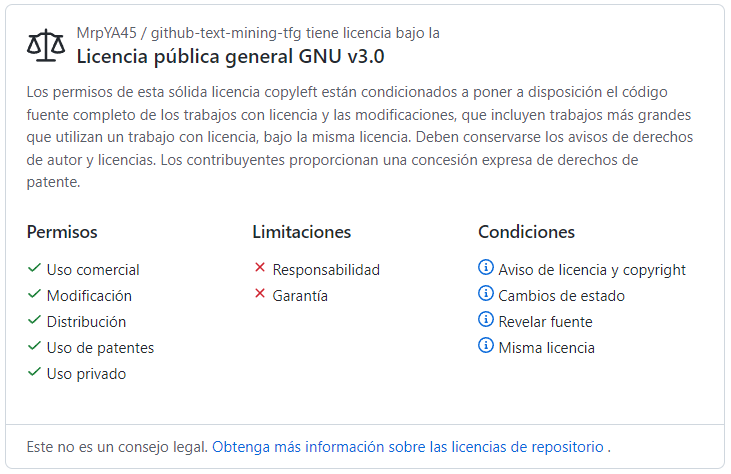
\includegraphics[width=\textwidth]{img/licencia_GNUGPLv3.png}
	\caption{Características de GNU General Public License v3.0 disponibles en el repositorio del proyecto \cite{vl:project-license-2021}.}
	\label{fig:gnu-gplv3}
\end{figure}

\subsubsection{Dependencias}

En esta sección se han recopilado y listado todas aquellas dependencias desarrolladas por terceros de las que se hace uso en el proyecto. Mediante el posterior cuadro se pone en conocimiento los complementos junto con sus correspondientes licencias de derechos de autor de estas para con su uso en el proyecto (véase \autoref{tabla:dependenciaslicencias}).

Todas las licencias incluidas en el proyecto cuentan con el grado necesario de compatibilidad entre ellas y con la propia licencia del proyecto, permitiendo distribuir y modificar el código fuente del proyecto siempre y cuando se mantenga una licencia compatible con todas ellas y con la propia licencia del proyecto.

\tablaSmall{Listado de dependencias con su correspondiente licencia}{p{4.5cm} p{2cm} p{5.2cm}}{dependenciaslicencias}
{ \multicolumn{1}{p{4.5cm}}{\raggedright\textbf{Dependencia}} & \multicolumn{1}{p{2cm}}{\raggedright\textbf{Versión}} & \multicolumn{1}{p{5cm}}{\raggedright\textbf{Licencia}}\\}{ 
    \emph{Python}                           & 3.9.6  & PSF License Agreement \cite{vl:python-software-foundation-2001}\\
    \emph{ReactJS}                          & 17.0.2 & MIT License \cite{vl:mit-license-1988}\\
    \emph{beautifulsoup4}                   & 4.9.3  & MIT License \\
    \emph{blingfire}                        & 0.1.7  & MIT License \\
    \emph{flask}                            & 2.0.1  & BSD-3-Clause Source License \cite{vl:bsd-3-clause-1988}\\
    \emph{flask-cors}                       & 3.0.10 & MIT License \\
    \emph{markdown}                         & 3.3.4  & BSD-3-Clause Source License \\
    \emph{markdown-checklist}               & 0.4.3  & BSD-3-Clause Source License \\
    \emph{mdx-gh-links}                     & 0.2    & BSD-3-Clause Source License \\
    \emph{nltk}                             & 3.6.2  & Apache License 2.0 \cite{vl:apache-2.0-2004}\\
    \emph{numpy}                            & 1.21.2 & BSD-3-Clause Source License \\
    \emph{pygithub}                         & 1.55   & GNU LGPL v3.0 \cite{vl:lgplv3}\\
    \emph{sqlalchemy}                       & 1.4.23 & MIT License \\
    \emph{torch}                            & 1.9.0  & Apache CLA \cite{vl:apache-cla}\\
    \emph{transformers}                     & 4.9.2  & Apache License 2.0 \\
    \emph{react-anchor-link-smooth-scroll}  & 1.0.12 & MIT License \\
    \emph{react google charts}              & 3.0.15 & MIT License \\
    \emph{react-helmet}                     & 6.1.0  & MIT License \\
    \emph{react-toastify}                   & 8.0.1  & MIT License \\
    \emph{react-hook-form}                  & 7.14.0 & MIT License \\
    \emph{wouter}                           & 2.7.4  & ISC License \cite{vl:isc-license-1995}\\
}


\apendice{Especificación de Requisitos}

\section{Introducción}

\section{Objetivos generales}

\section{Catalogo de requisitos}

\section{Especificación de requisitos}



\apendice{Especificación de diseño}

\section{Introducción}

El apéndice de especificación de diseño tiene como objetivo presentar al lector los aspectos del proyecto relativos al diseño de datos, el diseño procedimental y el diseño arquitectónico empleados en la aplicación.

El apartado de \hyperref[sec:datadesign]{diseño de datos} tiene como objetivo señalar el diseño de las entidades utilizado para el almacenamiento de la información manejada por la aplicación. La sección del \hyperref[sec:proceduraldesign]{diseño procedimental} introduce los flujos de interacción del usuario con la aplicación y entre sus componentes para la realización de las acciones planteadas en el apartado de requisitos funcionales. Finalmente el capítulo de \hyperref[sec:archdesign]{diseño arquitectónico} presenta la estructuración de los diversos componentes de la aplicación de acuerdo con el uso de una arquitectura de microservicios.

\section{Diseño de datos} \label{sec:datadesign}

El diseño de datos de la aplicación se ha diseñado a través del uso del ORM (Object–Relational Mapping) para Python SQLAlchemy conectado la aplicación con una base de datos de MariaDB. La utilización de un ORM facilita la interacción de los componentes de la aplicación con la base de datos, permitiendo interactuar con los datos de manera sencilla a través de objetos que actúan como intermediarios en el intercambios de la información.

En el diagrama relacional que se presenta a continuación (véase \autoref{fig:er_diagram}), se pueden observar las relaciones entre las entidades utilizadas por la aplicación, así como los atributos que estas entidades manejan. 

Las entidades ''Repositorio'', ''Incidencia'' y ''Comentario'' representan la manera en la que la información extraída desde GitHub por la aplicación es almacenada en la base de datos. Los repositorios almacenan el nombre, descripción y etiquetas que estos poseen. Los repositorios pueden mantener múltiples incidencias de las cuales se almacena su autor, título, descripción, etiquetas y un parámetro que nos indica si esa incidencia se corresponde con una petición de incorporación de cambios o no. A su vez, las incidencias pueden disponer de comentarios de los cuales se almacena su autor y la información del propio comentario.

\begin{figure}[!ht]
	\centering
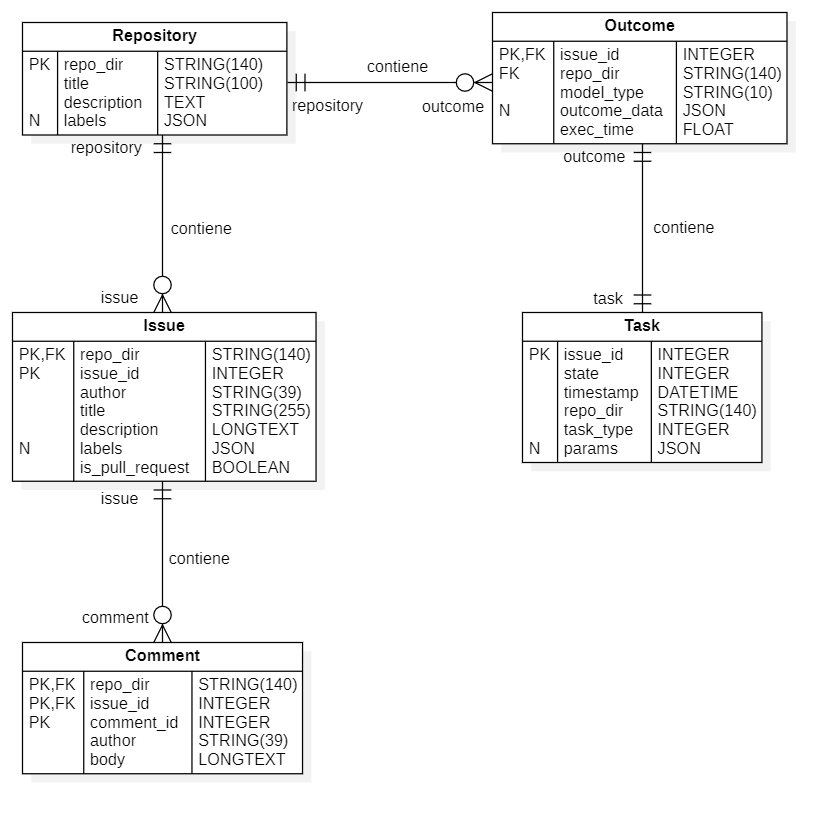
\includegraphics[width=\textwidth]{img/er_diagram.png}
	\caption{Esquema relacional de la base de datos.}
	\label{fig:er_diagram}
\end{figure}

La entidad ''Tarea'' representa la manera en la que se ha decidido generar la interacción entre los componentes del sistema. Con el objetivo de manejar y mantener un registro de las acciones llevadas a cabo por la aplicación se recurrió al uso de entidades ''Tarea'' para establecer una comunicación entre los componentes de la aplicación. Los servicios que componen la aplicación mantienen un proceso que consulta la base de datos de manera periódica en busca de tareas que concuerden con su objetivo y se mantengan en un estado a la espera de ser procesadas.

Finalmente, se puede observar una entidad ''Salida'' que representa los resultados de los experimentos lanzados. Mediante esta entidad se almacenan los resultados obtenidos posteriormente a la aplicación de los modelos de procesamiento del lenguaje natural, así como el tipo de modelo aplicado y el tiempo de ejecución que ha sido requerido para la obtención del resultado. Las salidas se relacionan con el repositorio cuyos datos han sido empleados para la aplicación del modelo.

\section{Diseño procedimental} \label{sec:proceduraldesign}

El diseño procedimental de la aplicación se presenta en el siguiente apartado a partir de los principales flujos de actividad que se desencadenan entre los componentes de la aplicación al lanzar las peticiones contra la API REST.

Podemos distinguir dos actividades fundamentales en la aplicación, las cuales son: la obtención de la información de los repositorios a partir de GitHub (véase \autoref{fig:sec_diagram_extract_repo}), y el lanzamiento de experimentos contra los datos extraídos de los repositorios (véase \autoref{fig:sec_diagram_run_experiment}). Ambos procesos se presentan en los siguientes diagramas de actividad. 

La comunicación entre procesos viene dada mediante dos tipos de relaciones: síncronas, representadas mediante flechas cuyo extremo se encuentra relleno, y asíncronas, representadas por flechas cuyo extremo solo se encuentra delineado. En cuanto a los recuadros de alternancia, representan los flujos de actividad alternativos producidos en función del resultado obtenido por la realización de una llamada.

\begin{sidewaysfigure}[!ht]
	\centering
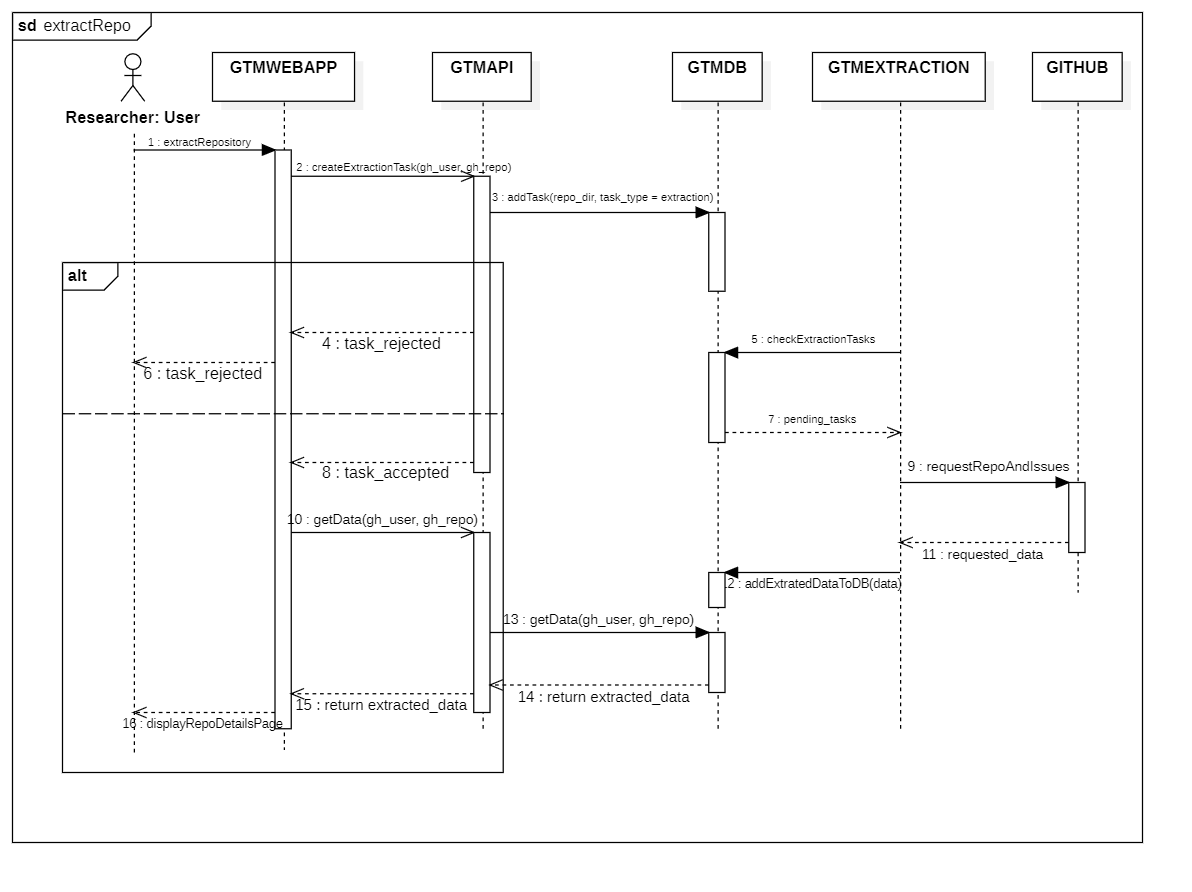
\includegraphics[width=\textwidth]{img/sec_diagram_extract_repo.png}
	\caption{Diagrama de secuencia correspondiente a la extracción de los datos de un repositorio.}
	\label{fig:sec_diagram_extract_repo}
\end{sidewaysfigure}

\begin{sidewaysfigure}[!ht]
	\centering
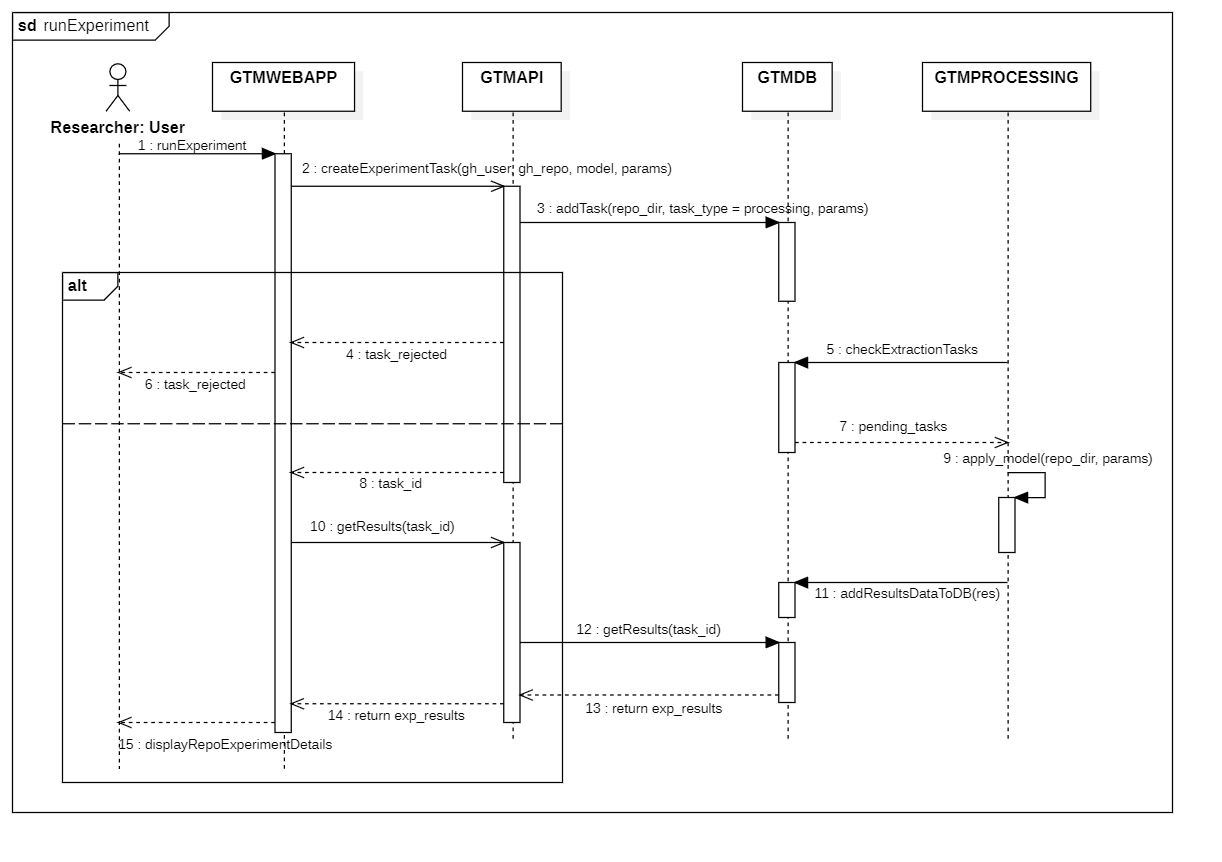
\includegraphics[width=\textwidth]{img/sec_diagram_run_experiment.png}
	\caption{Diagrama de secuencia genérico correspondiente al lanzamiento de un experimento.}
	\label{fig:sec_diagram_run_experiment}
\end{sidewaysfigure}

\clearpage
\section{Diseño arquitectónico} \label{sec:archdesign}

El diseño arquitectónico sobre el que se ha basado la estructura del proceso surge con la finalidad de fraccionar el proceso objetivo en fases más simples que operen de manera independiente. Esta división de los procesos otorga una mayor flexibilidad a la hora de incorporar cambios en alguna de las secciones minimizando los posibles efectos colaterales. La arquitectura que responde a estas características resulta en la utilización de una arquitectura de microservicios como se ha venido mencionando en la memoria.

\subsection{Backend}

El \textit{backend} del proyecto se encuentra conformado por 4 paquetes que desempeñan las funciones requeridas para el cumplimiento con los requisitos funcionales definidos previamente. Estos paquetes son el paquete \textit{gtmcore}, el paquete gtmapi, el paquete \textit{gtmextraction} y el paquete \textit{gtmprocessing}. La estructura interior de los paquetes sigue el esquema reducido de una arquitectura Modelo-Vista-Controlador (MVC) debido a que se enfoca en la estructuración de su código de acuerdo con la generación de una dependencia entre los datos de la aplicación y su lógica. Escalando un nivel se aprecia la dependencia existente entre los paquetes gtmapi, \textit{gtmextraction} y \textit{gtmprocessing} con el servicio \textit{gtmcore}. Este paquete tiene como objetivo dotar a los diversos servicios de aquellas funcionalidades que les permiten interactuar con la información almacenada en la base de datos (véase \autoref{fig:package_diagram}).

\begin{figure}[!ht]
	\centering
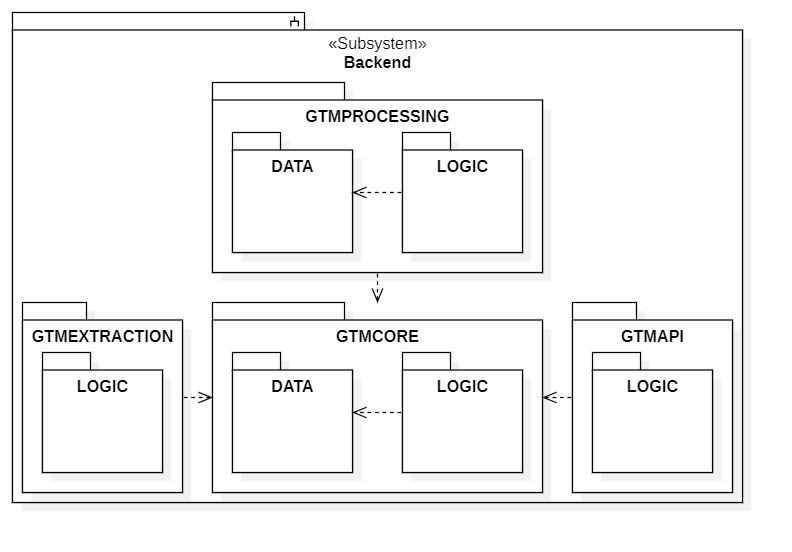
\includegraphics[width=\textwidth]{img/package_diagram.png}
	\caption{Diagrama de paquetes del proyecto.}
	\label{fig:package_diagram}
\end{figure}

Desde el punto de vista de los componentes lógicos que conforman el backend del proyecto, este se divide en cuatro servicios que podemos distinguir en función de su objetivo. El componente \textit{gtmapi} tiene como objetivo generar la interacción de la aplicación con el exterior, sea un usuario u otra aplicación que solicita sus servicios. El componente \textit{gtmextraction} tiene como finalidad establecer la conexión con GitHub y proceder a la extracción de la información de los repositorios. El componente \textit{gtmprocessing} tiene como propósito aplicar los modelos de procesamiento del lenguaje natural sobre la información extraída. Finalmente, el componente de la base de datos actúa como punto de interacción entre los servicios así como de almacén de la información (véase \autoref{fig:component_diagram}).

\begin{figure}[!ht]
	\centering
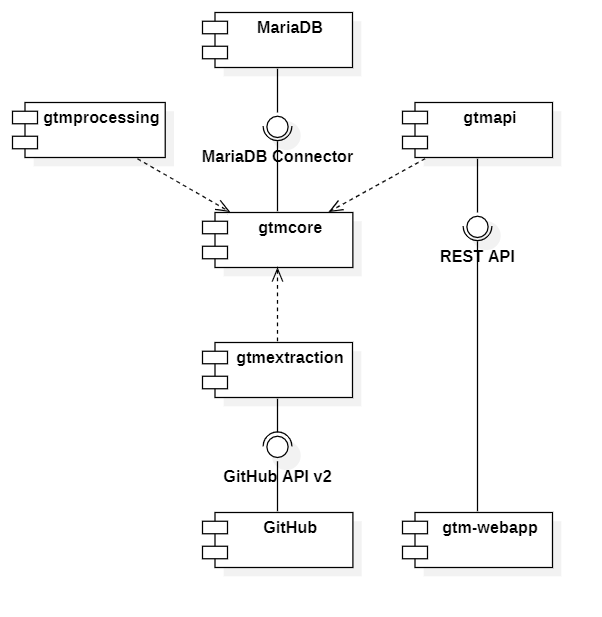
\includegraphics[width=\textwidth]{img/component_diagram.png}
	\caption{Diagrama de componentes del proyecto.}
	\label{fig:component_diagram}
\end{figure}

Acudiendo al diagrama de despliegue se puede observar la distribución física de los componentes de acuerdo con el mecanismo de despliegue que se ha decido utilizar. Los servicios se lanzan de manera aislada por medio de contenedores Docker. Esta distribución permite desplegar desde un mismo equipo varios SO aislados simulando su despliegue en varios equipos diferentes. Según las necesidades de recursos y distribución del proyecto el proyecto podría ser configurado para su despliegue en equipos diferentes siempre y cuando se respeten las vías de comunicación establecidas (véase \autoref{fig:deployment_diagram}).

\begin{figure}[!ht]
	\centering
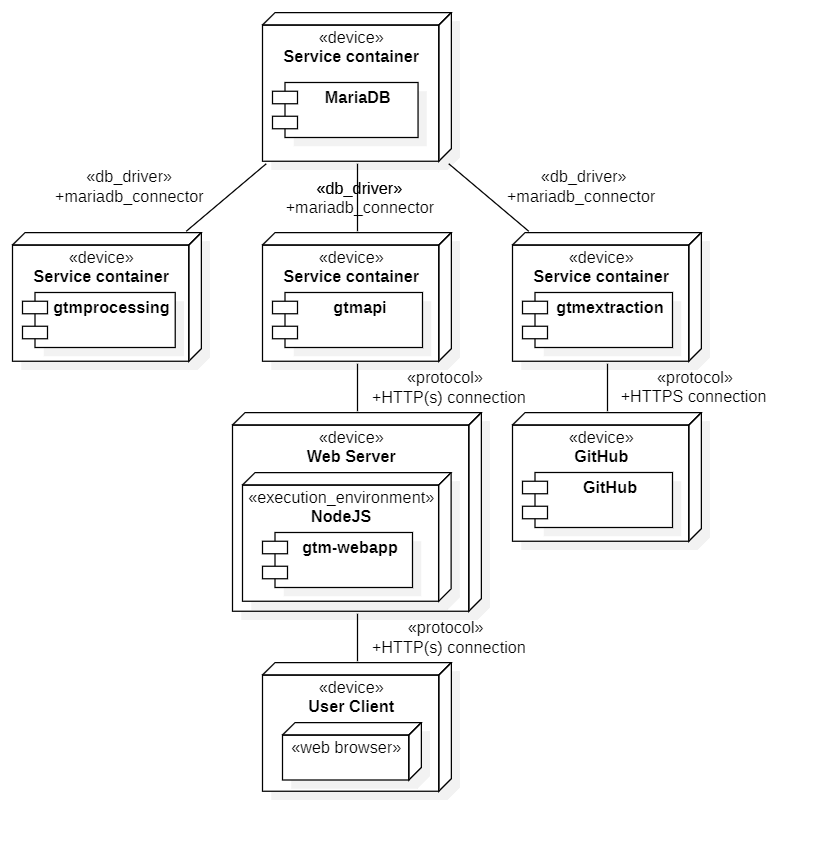
\includegraphics[width=\textwidth]{img/deployment_diagram.png}
	\caption{Diagrama de despliegue que refleja la arquitectura de microservicios implementada en el proyecto.}
	\label{fig:deployment_diagram}
\end{figure}

\subsection{Patrones de Diseño}

\subsubsection{Estrategia}

El patrón estrategia ha sido utilizado en el paquete de \textit{gtmprocessing} con el objetivo de facilitar la ampliación del número de modelos de procesamiento de lenguaje natural implementados en un futuro. El desarrollo se ha producido estableciendo una clase \textit{Project Manager} como Cliente que hace uso de los diferentes modelos (Estrategias) a través de la abstracción Base Model (véase \autoref{fig:class_diagram_processing}).

El uso de la abstracción requiere a sus descendientes de la implementación fundamental de los métodos \texttt{preprocess} y \textit{apply} entre otros. Estos métodos permiten a las subclases personalizar la adaptación necesaria de los datos al formato requerido por las entradas de los modelos. 

\begin{figure}[!ht]
	\centering
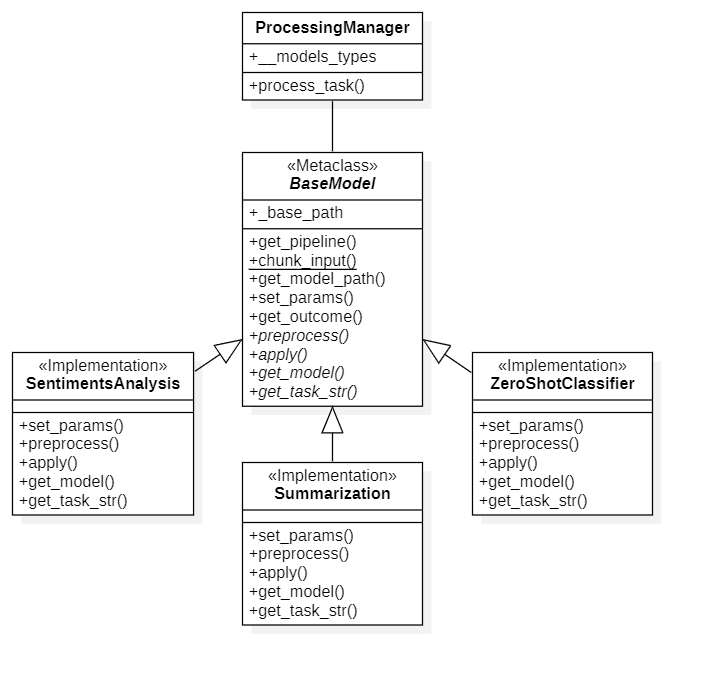
\includegraphics[width=\textwidth]{img/class_diagram_processing.png}
	\caption{Diagrama de clases de la lógica del procesamiento.}
	\label{fig:class_diagram_processing}
\end{figure}

Una particularidad del proceso de desarrollo realizado implica que el patrón estrategia no se ha desarrollado por completo debido a que si así fuese el patrón requeriría que la clase cliente no debería sufrir modificaciones ante la incorporación de nuevos modelos. En este caso, el cliente mantiene un diccionario que asocia una serie de claves con las diferentes implementaciones de los modelos. Pese a esta sutil diferencia, el cliente no requiere de modificaciones en su flujo de actividad principal que puedan alterar el comportamiento de la aplicación y causar puntos de fallo de mayor gravedad.

\apendice{Documentación técnica de programación}

\section{Introducción}

En el siguiente apéndice se incluye información relevante acerca de como se encuentran estructurados los directorios que componen el proyecto, así como las instrucciones de compilación, instalación y ejecución del proyecto.

\section{Estructura de directorios}

\subsection{Estructura directorio raíz}

En el directorio raíz podemos encontrar los contenidos del proyecto agrupados conforme a los siguientes directorios:

\begin{itemize} [\textbullet]
    \item \textbf{\texttt{.github/workflows}} Contiene los ficheros correspondientes los \emph{scripts} que configuran las \textbf{GitHub Actions} del repositorio.
    \item \textbf{\texttt{/docker}} Contiene los ficheros utilizados para la configuración y compilación de los contenedores \textbf{Docker}.
    \item \textbf{\texttt{/docs}} Contiene los ficheros fuente de \LaTeX utilizados para la generación de la documentación, incluyendo las imágenes utilizadas y las versiones finales de la memoria y sus anexos.
    \item \textbf{\texttt{/prototypes}} Contiene una \textbf{prueba de concepto} de la extracción de información desde GitHub implementada en un \emph{cuaderno de \textbf{Jupyter}}, así como una serie de ficheros que contienen los datos extraídos en las pruebas.
    \item \textbf{\texttt{/scripts}} Contiene una serie de scripts tanto para Windows como para Linux que permiten medir la calidad del código mediante la realización de comprobaciones de estilo y tipado sobre el código. Son utilizados por las \textbf{GitHub Actions}.
    \item \textbf{\texttt{/src}} Contiene el código fuente del proyecto dividido en dos directorios que separan el \hyperref[mp:backend]{back-end} del \hyperref[mp:front-end]{front-end}.
\end{itemize}

\subsection{Estructura de directorios del back-end} \label{mp:backend}

\begin{itemize} [\textbullet]
    \item \textbf{\texttt{/gtmapi}} Contiene los ficheros correspondientes al servicio de API REST de la plataforma. Proporciona un acceso al sistema desde el exterior mediante el cual otras aplicaciones puedan interactuar con él.
    \item \textbf{\texttt{/gtmcore}} Contiene una serie de ficheros de utilidad requeridos para el funcionamiento del resto de servicios. Incluye la implementación de un ORM a través del cual los servicios interactúan con la base de datos.
    \item \textbf{\texttt{/gtmextraction}} Contiene los ficheros correspondientes al servicio de extracción de datos de la plataforma. Incluye las clases encargadas de establecer la conexión con GitHub.
    \item \textbf{\texttt{/gtmprocessing}} Contiene los ficheros correspondientes al servicio de procesamiento de la plataforma. Incluye la implementación de una serie de clases que permiten leer los parámetros de los experimentos, solicitar la información requerida, aplicar los modelos preentrenados y almacenar los resultados obtenidos en la base de datos.
\end{itemize}

\subsection{Estructura de directorios de la webapp} \label{mp:front-end}
Contiene todos los ficheros relacionados con la aplicación web desarrollada con el framework \textbf{React}. En esta carpeta raíz se incluye el fichero ''package.json'' que contiene las dependencias necesarias para la instalación de la web.

\begin{itemize} [\textbullet]
    \item \textbf{\texttt{/public}} Contiene una serie de ficheros relacionados con el favicon de la web.
    \item \textbf{\texttt{/src}} Contiene los ficheros de \textbf{JavaScript} que dotan a la web de sus funciones, y los ficheros \textbf{CSS} que le proporcionan su apariencia.
    \begin{itemize} [\textbullet]
        \item \textbf{\texttt{/components}} Agrupa los componentes de React desarrollados para su uso en la aplicación.
        \item \textbf{\texttt{/images}} Contiene las imágenes utilizadas en la web. 
        \item \textbf{\texttt{/pages}} Contiene las vistas de la aplicación.
        \item \textbf{\texttt{/services}} Fundamentalmente contiene los scripts necesarios para lanzar peticiones contra la API REST.
    \end{itemize}
\end{itemize}

\section{Manual del programador}

El manual del programador tiene como objetivo ayudar a comprender a los futuros programadores interesados en continuar con el desarrollo del proyecto las indicaciones necesarias para hacer uso de las llamadas contra la API REST de la aplicación, así como indicios de cómo incorporar nuevos modelos de procesamiento del lenguaje natural sobre las bases que proporciona la aplicación.

\subsection{Uso de la API REST}

En la siguiente sección se incluye un listado de los endpoint proporcionados por la API junto con los parámetros necesarios para

\subsubsection{GET - Obtener estado}

\begin{itemize} \setlength\itemsep{0.2em}
    \item[] \textbf{Respuestas}
    \begin{itemize} \setlength\itemsep{0.2em}
        \item[] \textbf{200 OK}. La aplicación se está ejecutando.
    \end{itemize}
\end{itemize}

\subsubsection{GET - Obtener listado de las tareas}

\begin{itemize}
    \item[] \textbf{Ruta}
        \begin{itemize} \setlength\itemsep{0.2em}
            \item[] \texttt{/tasks/}
        \end{itemize}
    \item[] \textbf{Respuestas}
        \begin{itemize} \setlength\itemsep{0.2em}
            \item[] \textbf{200 OK}. Se obtiene un objeto JSON con un único atributo \textit{eqlts} que contiene un listado de objetos tarea.
                \begin{itemize} \setlength\itemsep{0.2em}
                    \item[] \textbf{Content-Type}: \texttt{application/json/}.
                    \item[] \textbf{Body}: 
                        \begin{itemize}
                            \item[] \textbf{task\_id}: Number
                            \item[] \textbf{state}: Number
                            \item[] \textbf{timestamp}: String
                            \item[] \textbf{repo\_dir}: String
                            \item[] \textbf{task\_type}: Number
                            \item[] \textbf{params}: Object
                        \end{itemize}
                \end{itemize}
            \item[] \textbf{500 Internal Server error}. Se ha producido un error interno en la aplicación.
        \end{itemize}
\end{itemize}

\subsubsection{GET - Obtener listado de los repositorios}

\begin{itemize}
    \item[] \textbf{Ruta}
        \begin{itemize} \setlength\itemsep{0.2em}
            \item[] \texttt{/repos/}
        \end{itemize}
    \item[] \textbf{Respuestas}
        \begin{itemize} \setlength\itemsep{0.2em}
            \item[] \textbf{200 OK}. Se obtiene un objeto JSON con un único atributo \textit{eqlts} que contiene un listado de objetos respositorio.
                \begin{itemize} \setlength\itemsep{0.2em}
                    \item[] \textbf{Content-Type}: \texttt{application/json/}.
                    \item[] \textbf{Body}: 
                        \begin{itemize} \setlength\itemsep{0.2em}
                            \item[] \textbf{repo\_dir}: String
                            \item[] \textbf{title}: String
                            \item[] \textbf{description}: String
                            \item[] \textbf{labels}: List
                        \end{itemize}
                \end{itemize}
            \item[] \textbf{500 Internal Server error}. Se ha producido un error interno en la aplicación.
        \end{itemize}
\end{itemize}

\subsubsection{GET - Obtener listado de las incidencias}

\begin{itemize}
    \item[] \textbf{Ruta}
        \begin{itemize} \setlength\itemsep{0.2em}
            \item[] \texttt{/issues/}
        \end{itemize}
    \item[] \textbf{Respuestas}
        \begin{itemize} \setlength\itemsep{0.2em}
            \item[] \textbf{200 OK}. Se obtiene un objeto JSON con un único atributo \textit{eqlts} que contiene un listado de objetos incidencia.
                \begin{itemize} \setlength\itemsep{0.2em}
                    \item[] \textbf{Content-Type}: \texttt{application/json/}.
                    \item[] \textbf{Body}: 
                        \begin{itemize} \setlength\itemsep{0.2em}
                            \item[] \textbf{repo\_dir}: String
                            \item[] \textbf{issue\_id}: Number
                            \item[] \textbf{author}: String
                            \item[] \textbf{title}: String
                            \item[] \textbf{description}: String
                            \item[] \textbf{labels}: List
                            \item[] \textbf{is\_pull\_request}: Boolean
                        \end{itemize}
                \end{itemize}
            \item[] \textbf{500 Internal Server error}. Se ha producido un error interno en la aplicación.
        \end{itemize}
\end{itemize}

\subsubsection{GET - Obtener listado de los comentarios}

\begin{itemize}
    \item[] \textbf{Ruta}
        \begin{itemize} \setlength\itemsep{0.2em}
            \item[] \texttt{/comments/}
        \end{itemize}
    \item[] \textbf{Respuestas}
        \begin{itemize} \setlength\itemsep{0.2em}
            \item[] \textbf{200 OK}. Se obtiene un objeto JSON con un único atributo \textit{eqlts} que contiene un listado de objetos comentario.
                \begin{itemize} \setlength\itemsep{0.2em}
                    \item[] \textbf{Content-Type}: \texttt{application/json/}.
                    \item[] \textbf{Body}: 
                        \begin{itemize} \setlength\itemsep{0.2em}
                            \item[] \textbf{repo\_dir}: String
                            \item[] \textbf{issue\_id}: Number
                            \item[] \textbf{comment\_id}: Number
                            \item[] \textbf{author}: String
                            \item[] \textbf{body}: String
                        \end{itemize}
                \end{itemize}
            \item[] \textbf{500 Internal Server error}. Se ha producido un error interno en la aplicación.
        \end{itemize}
\end{itemize}

\subsubsection{GET - Obtener listado de los resultados de las ejecuciones}

\begin{itemize}
    \item[] \textbf{Ruta}
        \begin{itemize} \setlength\itemsep{0.2em}
            \item[] \texttt{/outcomes/}
        \end{itemize}
    \item[] \textbf{Respuestas}
        \begin{itemize} \setlength\itemsep{0.2em}
            \item[] \textbf{200 OK}. Se obtiene un objeto JSON con un único atributo \textit{eqlts} que contiene un listado de objetos resultado.
                \begin{itemize} \setlength\itemsep{0.2em}
                    \item[] \textbf{Content-Type}: \texttt{application/json/}.
                    \item[] \textbf{Body}: 
                        \begin{itemize} \setlength\itemsep{0.2em}
                            \item[] \textbf{task\_id}: Number
                            \item[] \textbf{repo\_dir}: String
                            \item[] \textbf{model\_type}: String
                            \item[] \textbf{outcome\_data}: JSON
                            \item[] \textbf{exec\_time}: Number
                        \end{itemize}
                \end{itemize}
            \item[] \textbf{500 Internal Server error}. Se ha producido un error interno en la aplicación.
        \end{itemize}
\end{itemize}

\subsubsection{POST - Extraer la información de un repositorio}

\begin{itemize}
    \item[] \textbf{Ruta}
        \begin{itemize} \setlength\itemsep{0.2em}
            \item[] \texttt{/extract/}
        \end{itemize}
    \item[] \textbf{Parámetros}
        \begin{itemize} \setlength\itemsep{0.2em}
            \item[] \textbf{Content-Type}: \texttt{application/json/}.
            \item[] \textbf{Body}: 
                \begin{itemize} \setlength\itemsep{0.2em}
                    \item[] \textbf{gh\_user}: String
                    \item[] \textbf{gh\_repo}: String
                \end{itemize}
        \end{itemize}
    \item[] \textbf{Respuestas}
        \begin{itemize} \setlength\itemsep{0.2em}
            \item[] \textbf{200 OK}. Se obtiene un objeto JSON con un indicador de que la tarea ha sido encolada correctamente y su identificador único.
                \begin{itemize} \setlength\itemsep{0.2em}
                    \item[] \textbf{Content-Type}: \texttt{application/json/}.
                    \item[] \textbf{Body}: 
                        \begin{itemize} \setlength\itemsep{0.2em}
                            \item[] \textbf{Added}: [Body] Boolean
                            \item[] \textbf{task\_id}: [Body] Number
                        \end{itemize}
                \end{itemize}
            \item[] \textbf{400 Bad Request}. Los parámetros introducidos son incorrectos.
            \item[] \textbf{500 Internal Server error}. Se ha producido un error interno en la aplicación.
        \end{itemize}
\end{itemize}

\subsubsection{GET - Obtener la información de un repositorio}

\begin{itemize}
    \item[] \textbf{Ruta}
        \begin{itemize} \setlength\itemsep{0.2em}
            \item[] \texttt{/user/<string:gh\_user>/repo/<string:gh\_repo>}
        \end{itemize}
    \item[] \textbf{Parámetros}
        \begin{itemize} \setlength\itemsep{0.2em}
            \item[] \textbf{gh\_user}: [Path] String
            \item[] \textbf{gh\_repo}: [Path] String
        \end{itemize}
    \item[] \textbf{Respuestas}
        \begin{itemize} \setlength\itemsep{0.2em}
            \item[] \textbf{200 OK}. Se obtiene un objeto JSON con la información del repositorio.
                \begin{itemize} \setlength\itemsep{0.2em}
                    \item[] \textbf{Content-Type}: \texttt{application/json/}.
                    \item[] \textbf{Body}: 
                        \begin{itemize} \setlength\itemsep{0.2em}
                            \item[] \textbf{repo\_dir}: String
                            \item[] \textbf{title}: String
                            \item[] \textbf{description}: String
                            \item[] \textbf{labels}: List
                        \end{itemize}
                \end{itemize}
            \item[] \textbf{202 Accepted}. La petición es correcta pero la información solicitada aún no se encuentra disponible.
            \item[] \textbf{404 Not Found}. No se encuentra ningún repositorio de acuerdo con los parámetros introducidos.
            \item[] \textbf{424 Failed Dependency}. La extracción de los datos del repositorio falló.
            \item[] \textbf{500 Internal Server error}. Se ha producido un error interno en la aplicación.
        \end{itemize}
\end{itemize}

\subsubsection{GET - Obtener la información de una incidencia de un repositorio}

\begin{itemize}
    \item[] \textbf{Ruta}
        \begin{itemize} \setlength\itemsep{0.2em}
            \item[] \texttt{/user/<string:gh\_user>/repo/<string:gh\_repo>/issue/<int:issue\_id>}
        \end{itemize}
    \item[] \textbf{Parámetros}
        \begin{itemize} \setlength\itemsep{0.2em}
            \item[] \textbf{gh\_user}: [Path] String
            \item[] \textbf{gh\_repo}: [Path] String
            \item[] \textbf{issue\_id}: [Path] Number            
        \end{itemize}
    \item[] \textbf{Respuestas}
        \begin{itemize} \setlength\itemsep{0.2em}
            \item[] \textbf{200 OK}. Se obtiene un objeto JSON con la información de la incidencia.
                \begin{itemize} \setlength\itemsep{0.2em}
                    \item[] \textbf{Content-Type}: \texttt{application/json/}.
                    \item[] \textbf{Body}: 
                        \begin{itemize} \setlength\itemsep{0.2em}
                            \item[] \textbf{repo\_dir}: String
                            \item[] \textbf{issue\_id}: Number
                            \item[] \textbf{author}: String
                            \item[] \textbf{title}: String
                            \item[] \textbf{description}: String
                            \item[] \textbf{labels}: List
                            \item[] \textbf{is\_pull\_request}: Boolean
                        \end{itemize}
                \end{itemize}
            \item[] \textbf{400 Bad Request}. Los parámetros introducidos son incorrectos.
            \item[] \textbf{404 Not Found}. No se encuentra ninguna incidencia de acuerdo con los parámetros introducidos.
            \item[] \textbf{500 Internal Server error}. Se ha producido un error interno en la aplicación.
        \end{itemize}
\end{itemize}

\subsubsection{GET - Obtener las incidencias de un repositorio}

\begin{itemize}
    \item[] \textbf{Ruta}
        \begin{itemize} \setlength\itemsep{0.2em}
            \item[] \texttt{/user/<string:gh\_user>/repo/<string:gh\_repo>/issues}
        \end{itemize}
    \item[] \textbf{Parámetros}
        \begin{itemize} \setlength\itemsep{0.2em}
            \item[] \textbf{gh\_user}: [Path] String
            \item[] \textbf{gh\_repo}: [Path] String
        \end{itemize}
    \item[] \textbf{Respuestas}
        \begin{itemize} \setlength\itemsep{0.2em}
            \item[] \textbf{200 OK}. Se obtiene un objeto JSON con una lista incidencias del repositorio.
                \begin{itemize} \setlength\itemsep{0.2em}
                    \item[] \textbf{Content-Type}: \texttt{application/json/}.
                    \item[] \textbf{Body}: 
                        \begin{itemize} \setlength\itemsep{0.2em}
                            \item[] \textbf{repo\_dir}: String
                            \item[] \textbf{issue\_id}: Number
                            \item[] \textbf{author}: String
                            \item[] \textbf{title}: String
                            \item[] \textbf{description}: String
                            \item[] \textbf{labels}: List
                            \item[] \textbf{is\_pull\_request}: Boolean
                        \end{itemize}
                \end{itemize}
            \item[] \textbf{202 Accepted}. La petición es correcta pero la información solicitada aún no se encuentra disponible.
            \item[] \textbf{404 Not Found}. No se encuentra ningún repositorio de acuerdo con los parámetros introducidos.
            \item[] \textbf{424 Failed Dependency}. La extracción de los datos del repositorio falló.
            \item[] \textbf{500 Internal Server error}. Se ha producido un error interno en la aplicación.
        \end{itemize}
\end{itemize}

\subsubsection{GET - Obtener los comentarios de una incidencia}

\begin{itemize}
    \item[] \textbf{Ruta}
        \begin{itemize} \setlength\itemsep{0.2em}
            \item[] \texttt{/user/<string:gh\_user>/repo/<string:gh\_repo>/issue/<int:issue\_id>/comments}
        \end{itemize}
    \item[] \textbf{Parámetros}
        \begin{itemize} \setlength\itemsep{0.2em}
            \item[] \textbf{gh\_user}: [Path] String
            \item[] \textbf{gh\_repo}: [Path] String
            \item[] \textbf{issue\_id}: [Path] Number
        \end{itemize}
    \item[] \textbf{Respuestas}
        \begin{itemize} \setlength\itemsep{0.2em}
            \item[] \textbf{200 OK}. Se obtiene un objeto JSON con una lista comentarios de la incidencia.
                \begin{itemize} \setlength\itemsep{0.2em}
                    \item[] \textbf{Content-Type}: \texttt{application/json/}.
                    \item[] \textbf{Body}: 
                        \begin{itemize} \setlength\itemsep{0.2em}
                            \item[] \textbf{repo\_dir}: String
                            \item[] \textbf{issue\_id}: Number
                            \item[] \textbf{author}: String
                            \item[] \textbf{title}: String
                            \item[] \textbf{description}: String
                            \item[] \textbf{labels}: List
                            \item[] \textbf{is\_pull\_request}: Boolean
                        \end{itemize}
                \end{itemize}
            \item[] \textbf{202 Accepted}. La petición es correcta pero la información solicitada aún no se encuentra disponible.
            \item[] \textbf{404 Not Found}. No se encuentra ningún repositorio de acuerdo con los parámetros introducidos.
            \item[] \textbf{424 Failed Dependency}. La extracción de los datos del repositorio falló.
            \item[] \textbf{500 Internal Server error}. Se ha producido un error interno en la aplicación.
        \end{itemize}
\end{itemize}

\subsubsection{GET - Obtener las operaciones realizadas sobre un repositorio}

\begin{itemize}
    \item[] \textbf{Ruta}
        \begin{itemize} \setlength\itemsep{0.2em}
            \item[] \texttt{/user/<string:gh\_user>/repo/<string:gh\_repo>/tasks}
        \end{itemize}
    \item[] \textbf{Parámetros}
        \begin{itemize} \setlength\itemsep{0.2em}
            \item[] \textbf{gh\_user}: [Path] String
            \item[] \textbf{gh\_repo}: [Path] String
        \end{itemize}
    \item[] \textbf{Respuestas}
        \begin{itemize} \setlength\itemsep{0.2em}
            \item[] \textbf{200 OK}. Se obtiene un objeto JSON con la lista de las operaciones realizadas sobre el repositorio.
                \begin{itemize} \setlength\itemsep{0.2em}
                    \item[] \textbf{Content-Type}: \texttt{application/json/}.
                    \item[] \textbf{Body}: 
                        \begin{itemize} \setlength\itemsep{0.2em}
                            \item[] \textbf{task\_id}: Number
                            \item[] \textbf{state}: Number
                            \item[] \textbf{timestamp}: String
                            \item[] \textbf{repo\_dir}: String
                            \item[] \textbf{task\_type}: Number
                            \item[] \textbf{params}: Object
                        \end{itemize}
                \end{itemize}
            \item[] \textbf{204 No Content}. No se localizan registros de repositorios que concuerden con los parámetros introducidos.
            \item[] \textbf{500 Internal Server error}. Se ha producido un error interno en la aplicación.
        \end{itemize}
\end{itemize}

\subsubsection{GET - Obtener los experimentos lanzados sobre un repositorio}

\begin{itemize}
    \item[] \textbf{Ruta}
        \begin{itemize} \setlength\itemsep{0.2em}
            \item[] \texttt{/user/<string:gh\_user>/repo/<string:gh\_repo>/experiments}
        \end{itemize}
    \item[] \textbf{Parámetros}
        \begin{itemize} \setlength\itemsep{0.2em}
            \item[] \textbf{gh\_user}: [Path] String
            \item[] \textbf{gh\_repo}: [Path] String
        \end{itemize}
    \item[] \textbf{Respuestas}
        \begin{itemize} \setlength\itemsep{0.2em}
            \item[] \textbf{200 OK}. Se obtiene un objeto JSON con la lista de los resultados de los experimentos lanzados sobre el repositorio.
                \begin{itemize} \setlength\itemsep{0.2em}
                    \item[] \textbf{Content-Type}: \texttt{application/json/}.
                    \item[] \textbf{Body}: 
                        \begin{itemize} \setlength\itemsep{0.2em}
                            \item[] \textbf{task\_id}: Number
                            \item[] \textbf{repo\_dir}: String
                            \item[] \textbf{model\_type}: String
                            \item[] \textbf{outcome\_data}: JSON
                            \item[] \textbf{exec\_time}: Number
                        \end{itemize}
                \end{itemize}
            \item[] \textbf{204 No Content}. No se localizan registros de repositorios que concuerden con los parámetros introducidos.
            \item[] \textbf{500 Internal Server error}. Se ha producido un error interno en la aplicación.
        \end{itemize}
\end{itemize}

\subsubsection{POST - Lanzar un experimento de Zero-Shot Classification sobre un repositorio}

\begin{itemize}
    \item[] \textbf{Ruta}
        \begin{itemize} \setlength\itemsep{0.2em}
            \item[] \texttt{/user/<string:gh\_user>/repo/<string:gh\_repo>/process/zsc/}
        \end{itemize}
    \item[] \textbf{Content-Type}: \texttt{application/json/}.
    \item[] \textbf{Parámetros}
        \begin{itemize} \setlength\itemsep{0.2em}
            \item[] \textbf{gh\_user}: [Path] String
            \item[] \textbf{gh\_repo}: [Path] String
            \item[] \textbf{issue\_id}: [Body] Number
            \item[] \textbf{accuracy}: [Body] Float. Entre 0 y 1.
            \item[] \textbf{use\_desc}: [Body] Boolean
            \item[] \textbf{extra\_labels}: [Body] String. Cada término deberá estar separado por un punto y coma.
        \end{itemize}
    \item[] \textbf{Respuestas}
        \begin{itemize} \setlength\itemsep{0.2em}
            \item[] \textbf{200 OK}. Se obtiene un objeto JSON con un indicador de que el experimento ha sido encolado correctamente y su identificador único.
                \begin{itemize} \setlength\itemsep{0.2em}
                    \item[] \textbf{Content-Type}: \texttt{application/json/}.
                    \item[] \textbf{Body}: 
                        \begin{itemize} \setlength\itemsep{0.2em}
                            \item[] \textbf{Added}: [Body] Boolean
                            \item[] \textbf{task\_id}: [Body] Number
                        \end{itemize}
                \end{itemize}
            \item[] \textbf{400 Bad Request}. Los parámetros introducidos son incorrectos.
            \item[] \textbf{406 Not Acceptable}. Los parámetros introducidos no se corresponden con ninguno de los repositorios disponibles.
            \item[] \textbf{500 Internal Server error}. Se ha producido un error interno en la aplicación.
            \item[] \textbf{503 Service Unavailable}. En estos momentos no es posible lanzar el experimento sobre el repositorio solicitado.
        \end{itemize}
\end{itemize}

\subsubsection{POST - Lanzar un experimento de Sentiment Analysis sobre un repositorio}

\begin{itemize}
    \item[] \textbf{Ruta}
        \begin{itemize} \setlength\itemsep{0.2em}
            \item[] \texttt{/user/<string:gh\_user>/repo/<string:gh\_repo>/process/sa/}
        \end{itemize}
    \item[] \textbf{Content-Type}: \texttt{application/json/}.
    \item[] \textbf{Parámetros}
        \begin{itemize} \setlength\itemsep{0.2em}
            \item[] \textbf{gh\_user}: [Path] String
            \item[] \textbf{gh\_repo}: [Path] String
            \item[] \textbf{issue\_id}: [Body] Integer
            \item[] \textbf{author}: [Body] String.
            \item[] \textbf{with\_comments}: [Body] Boolean
        \end{itemize}
    \item[] \textbf{Respuestas}
        \begin{itemize} \setlength\itemsep{0.2em}
            \item[] \textbf{200 OK}. Se obtiene un objeto JSON con un indicador de que el experimento ha sido encolado correctamente y su identificador único.
                \begin{itemize} \setlength\itemsep{0.2em}
                    \item[] \textbf{Content-Type}: \texttt{application/json/}.
                    \item[] \textbf{Body}: 
                        \begin{itemize} \setlength\itemsep{0.2em}
                            \item[] \textbf{Added}: [Body] Boolean
                            \item[] \textbf{task\_id}: [Body] Number
                        \end{itemize}
                \end{itemize}
            \item[] \textbf{400 Bad Request}. Los parámetros introducidos son incorrectos.
            \item[] \textbf{406 Not Acceptable}. Los parámetros introducidos no se corresponden con ninguno de los repositorios disponibles.
            \item[] \textbf{500 Internal Server error}. Se ha producido un error interno en la aplicación.
            \item[] \textbf{503 Service Unavailable}. En estos momentos no es posible lanzar el experimento sobre el repositorio solicitado.
        \end{itemize}
\end{itemize}

\subsubsection{POST - Lanzar un experimento de Summarization sobre un repositorio}

\begin{itemize}
    \item[] \textbf{Ruta}
        \begin{itemize} \setlength\itemsep{0.2em}
            \item[] \texttt{/user/<string:gh\_user>/repo/<string:gh\_repo>/process/summ/}
        \end{itemize}
    \item[] \textbf{Content-Type}: \texttt{application/json/}.
    \item[] \textbf{Parámetros}
        \begin{itemize} \setlength\itemsep{0.2em}
            \item[] \textbf{gh\_user}: [Path] String
            \item[] \textbf{gh\_repo}: [Path] String
            \item[] \textbf{max\_length}: [Body] Integer
            \item[] \textbf{min\_length}: [Body] Integer
            \item[] \textbf{with\_comments}: [Body] Boolean
        \end{itemize}
    \item[] \textbf{Respuestas}
        \begin{itemize} \setlength\itemsep{0.2em}
            \item[] \textbf{200 OK}. Se obtiene un objeto JSON con un indicador de que el experimento ha sido encolado correctamente y su identificador único.
                \begin{itemize} \setlength\itemsep{0.2em}
                    \item[] \textbf{Content-Type}: \texttt{application/json/}.
                    \item[] \textbf{Body}: 
                        \begin{itemize} \setlength\itemsep{0.2em}
                            \item[] \textbf{Added}: [Body] Boolean
                            \item[] \textbf{task\_id}: [Body] Number
                        \end{itemize}
                \end{itemize}
            \item[] \textbf{400 Bad Request}. Los parámetros introducidos son incorrectos.
            \item[] \textbf{406 Not Acceptable}. Los parámetros introducidos no se corresponden con ninguno de los repositorios disponibles.
            \item[] \textbf{500 Internal Server error}. Se ha producido un error interno en la aplicación.
            \item[] \textbf{503 Service Unavailable}. En estos momentos no es posible lanzar el experimento sobre el repositorio solicitado.
        \end{itemize}
\end{itemize}

\section{Instalación y ejecución del proyecto}

En el siguiente apartado se presentan las instrucciones a través de las cuales establecer un entorno de desarrollo que disponga del código fuente, utilidades, complementos y ejecutables requeridos para la puesta en marcha del proyecto. 

\subsection{Prerrequisitos}
El código fuente del proyecto se ha implementado haciendo uso de los lenguajes de programación \textbf{Python} y \textbf{JavaScript}. En el caso de Python este se requiere para las implementaciones llevadas a cabo en el apartado del front-end. El uso de JavaScript se debe al desarrollo de la aplicación web, implementada sobre el entorno de ejecución \textbf{NodeJS}. A continuación se incluyen las versiones requeridas por la aplicación para asegurar su correcto funcionamiento:
\begin{itemize}
    \item \textbf{Python 3.9.6} o superior.
    \item \textbf{NodeJS 14.17.4} o superior.
    \item \textbf{Docker 20.10.12} o superior.
    \item \textbf{Docker Compose 1.29.2} o superior.
\end{itemize}
Se recomienda el uso del editor de texto \textbf{Visual Studio Code} debido a la versatilidad que ofrece a la hora de trabajar con diversos lenguajes de manera simultánea y el uso de extensiones que facilitan múltiples aspectos en el proceso de desarrollo.

\subsection{Obtención el proyecto}

El proyecto se encuentra alojado en un repositorio de GitHub de acceso libre. Para proceder con la obtención de una copia local de los ficheros se recurrirá a un software de control de versiones que ofrezcan soporte a repositorios de GitHub como \textbf{Git} o \textbf{GitHub Desktop}. También es posible la descarga directa de los ficheros a través de la dirección de GitHub en la cual se encuentra alojado el repositorio. La dirección de acceso al repositorio es la siguiente:

\vspace{0.5cm}
\centerline{\texttt{\url{https://github.com/MrpYA45/github-text-mining-tfg}}}
\vspace{0.4cm}

En caso de que se haya decidido escoger el popular software de control de versiones Git el comando requerido para la obtención de los archivos es el siguiente:

\vspace{0.5cm}
\centerline{\texttt{git clone https://github.com/MrpYA45/github-text-mining-tfg}}
\vspace{0.4cm}

\begin{figure}[!ht]
	\centering
    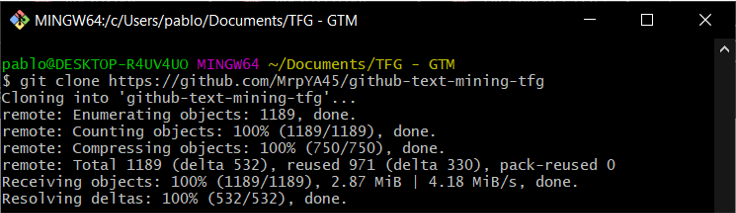
\includegraphics[width=\textwidth]{img/git_gtm.png}
	\caption{Obtención del repositorio mediante Git.}
	\label{fig:git_gtm_mp}
\end{figure}

\subsection{Preparación de un entorno virtual}

Los entornos virtuales de Python permiten mantener varios desarrollos en el mismo equipo de manera que las configuraciones y dependencias de un entorno se mantengan aisladas del resto de entornos virtuales. No es un requisito obligatorio su uso pero sí recomendable para evitar conflictos entre posibles múltiples versiones de las dependencias utilizadas entre proyectos, manteniendo solo aquellas estrictamente necesarias para el desarrollo. 

Para crear un entorno virtual se deberá situar la terminal en el directorio raíz del proyecto y ejecutar el comando dispuesto a continuación:

\vspace{0.5cm}
\centerline{\textbf{MacOS/Linux:} \texttt{python3 -m venv env}}
\centerline{\textbf{Windows:} \texttt{python -m venv env}}
\vspace{0.4cm}

\begin{figure}[!ht]
	\centering
    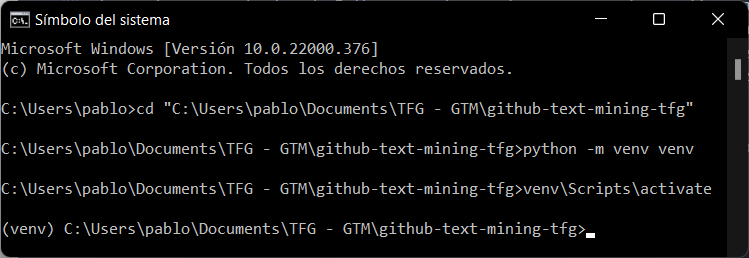
\includegraphics[width=\textwidth]{img/creating_venv.png}
	\caption{Creación de un entorno virtual para Python.}
	\label{fig:python_venv_creation}
\end{figure}

Una vez se disponga de un entorno virtual deberemos activarlo, para la cual el comando a utilizar dependerá del sistema operativo que se vaya a utilizar (véase \autoref{fig:python_venv_creation}).

\vspace{0.5cm}
\centerline{\textbf{MacOS/Linux:} \texttt{source venv/bin/activate}}
\centerline{\textbf{Windows:} \texttt{venv\textbackslash Scripts\textbackslash activate}}
\vspace{0.4cm}

\subsection{Instalación de las dependencias del back-end}
Seguidamente se realizará la instalación de las dependencias de Python utilizadas en el proyecto de acuerdo con el listado de paquetes que se proporciona en el directorio raíz del proyecto mediante el fichero \texttt{requirements.txt}. La instalación se realizará a través del gestor de paquetes \textbf{PIP}, el cual se distribuye junto con Python desde la versión 3.4.

\vspace{0.5cm}
\centerline{\textbf{MacOS/Linux:} \texttt{pip3 install -r requirements.txt}}
\centerline{\textbf{Windows:} \texttt{pip install -r requirements.txt}}
\vspace{0.4cm}

\subsection{Instalación de las dependencias de la aplicación web}
A continuación, se procederá con la instalación de las dependencias de la aplicación web. Esta se encuentra construida sobre el entorno de ejecución NodeJS basado en JavaScript. La aplicación web también ha sido desarrollada haciendo uso de módulos que simplifican la programación de ciertos aspectos de la web.

Para proceder a la instalación de estas dependencias se deberá situar la terminal en la carpeta \texttt{src/webapp}. El fichero \texttt{package.json} es el encargado de almacenar el listado con las dependencias necesarias para poder proceder con la instalación, así como los \textit{scripts} que permiten lanzar la aplicación. Para proceder con la instalación de los ficheros necesarios se deberá recurrir al siguiente comando:

\vspace{0.5cm}
\centerline{\textbf{Windows/MacOS/Linux: } \texttt{npm install}}
\vspace{0.4cm}

\subsection{Lanzamiento de los servicios del back-end}

El lanzamiento de los servicios del back-end se realizará por medio del uso de las herramientas \textbf{Docker} y \textbf{Docker Compose}, para las cuales se ha diseñado una configuración que permite mantener cada uno de los servicios y la base de datos en contenedores independientes.

El primer paso consistirá en la obtención de las imágenes que se ejecutarán en el interior de los contenedores. Para ello, situándonos en la directorio raíz del proyecto, se deberá ejecutar el comando de construcción que se incluye a continuación. Se ha de tener en cuenta que la primera ejecución del comando requiere de la descarga de numerosos archivos pesados, por ello por lo que el proceso puede alargarse durante varios minutos.

\vspace{0.5cm}
\centerline{\textbf{Windows/MacOS/Linux:}}
\centerline{\texttt{docker-compose -f docker/config/docker-compose.yml build}}
\vspace{0.4cm}

Una vez se ha completado el proceso de generación de las imágenes se deberá proseguir con el levantamiento de los contenedores que contendrán dichas imágenes. En una primera instancia este proceso requiere de un extenso tiempo de espera durante el cual se procede a la descarga e instalación de las dependencias requeridas por los servicios en el interior de los propios contenedores.

\vspace{0.5cm}
\centerline{\textbf{Windows/MacOS/Linux:}}
\centerline{\texttt{docker-compose -f docker/config/docker-compose.yml up}}
\vspace{0.4cm}

El servicio con un mayor tiempo de despliegue inicial resulta ser el servicio de procesamiento denominado \textit{gtmprocessing}, el cual puede llegar a requerir de entre 10 y 15 minutos en su arranque. Ante la pobre vivacidad que se presenta en el proceso de obtención de los modelos se recomienda realizar comprobaciones periódicas a través del siguiente comando.

\vspace{0.5cm}
\centerline{\textbf{Windows/MacOS/Linux: } \texttt{docker logs gtmprocessing -t}}
\vspace{0.4cm}

Esta orden permite obtener un visualizar la actividad que se está produciendo en el interior del contenedor. A través de esta salida se podrá comprobar el estado de la descarga de los modelos.

\subsubsection{Configuración inicial de los servicios}

Una vez finalizado el proceso de configuración inicial se deberá verificar que se han generado correctamente los ficheros de configuración. Estos ficheros se encuentran en el interior de cada uno de los servicios en la ruta \texttt{/src/backend/\%service\_name\%/config}.

Verificada la existencia de estos ficheros se deberán detener los contenedores para poder proceder a su pertinente configuración.

\vspace{0.5cm}
\centerline{\textbf{Windows/MacOS/Linux:}}
\centerline{\texttt{docker-compose -f docker/config/docker-compose.yml stop}}
\vspace{0.4cm}

Cada servicio dispone de una carpeta \textit{gtmcore} en su configuración que permite alterar los parámetros de conexión con la base de datos. Por defecto, estos ficheros se generan con una configuración básica de acuerdo con la configuración de la base de datos establecida en el fichero de variables de entorno de Docker localizado en la siguiente ruta \texttt{docker/services/.env}. Se recomienda encarecidamente modificar estos valores en caso de lanzar la aplicación en algún entorno de producción.

Finalmente, el servicio de extracción dispone de una segunda carpeta de configuración denominada \textit{gtmprocessing}. En su interior se encuentra un fichero de configuración que se requiere completar para lograr la extracción de la información de los repositorios. Este fichero solicita un token de acceso personal de GitHub.

Una vez se haya completado la configuración de los servicios se deberá volver a levantar los contenedores con el comando señalado anteriormente. En el momento en que los servicios se encuentren completamente desplegados será posible acceder a la API REST de la aplicación por medio de consultas a la dirección \url{http://localhost:6060/}.

\subsubsection{Obtención de un token de acceso personal de GitHub}

La obtención de un token de acceso personal de GitHub requiere de encontrarnos registrados en la plataforma. Una vez en ella se puede solicitar el token desde el apartado de \textit{Settings}, \textit{Developer Settings}, y seleccionar el apartado \href{https://github.com/settings/tokens}{\textit{Personal Access Tokens}}.

La generación de un token requiere del establecimiento de un periodo de caducidad y de la selección de una serie de permisos básicos para poder realizar ciertas acciones. El uso básico de las peticiones que se realizan por parte de la aplicación implica que solo se requiere del permiso de acceso a repositorios públicos (véase \autoref{fig:gen_github_access_tokens_mp}).

\begin{figure}[!ht]
	\centering
    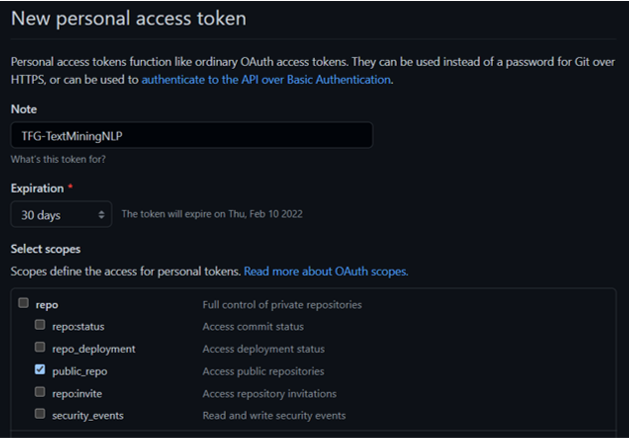
\includegraphics[width=\textwidth]{img/gen_github_access_tokens.png}
	\caption{Generación del Token de Acceso Personal en GitHub.}
	\label{fig:gen_github_access_tokens_mp}
\end{figure}

\subsection{Lanzamiento de la aplicación web mediante NodeJS}

El lanzamiento de aplicación web solamente requiere de la situación de la terminal en la ruta donde se localiza los ficheros de la aplicación web (\texttt{src/webapp}) y la introducción del siguiente comando. 

\vspace{0.5cm}
\centerline{\textbf{Windows/MacOS/Linux: } \texttt{npm start gtm-webapp}}
\vspace{0.4cm}

Tras su ejecución se producirá el despliegue de la aplicación en un servidor de NodeJS y la apertura automática de una ventana en el navegador web presentando al usuario la web. En caso de que esto no suceda por algún motivo desconocido, la aplicación web se encuentra accesible desde la siguiente dirección \url{http://localhost:3000/}.

\section{Pruebas del sistema}

Las pruebas de sistema permiten comprobar la robustez de este mediante el sometimiento del sistema a métricas o situaciones que verifiquen la respuesta de este ciertas condiciones cumpliendo con los requisitos establecidos. Durante el desarrollo del proyecto se destaca el uso de dos tipos de pruebas: pruebas de calidad de código y pruebas de comportamiento. 

\subsection{Métricas de calidad de código y documentación}

La verificación de la calidad del código se ha llevado a cabo a partir del uso de las herramientas \textbf{Pylint} y \textbf{MyPy} de Python cuyo objetivo consiste en comprobar que el código se adapta unos estándares de calidad adecuados. Ambas herramientas han sido utilizadas por medio de ficheros ejecutables que se encuentran accesibles en la carpeta \textit{scripts} del proyecto.

El paquete Pylint se encarga de comprobar y verificar que el código y su documentación se adapta a la guía de estilo \textbf{PEP 8} (Python Enhancement Proposal 8). Las comprobaciones realizadas por esta herramienta se basan en calificar multitud de escenarios y dotar al proyecto de una puntuación de acuerdo con dichas métricas de calidad.

El paquete MyPy tiene como objetivo comprobar que se hace un buen uso de los tipos estáticos recientemente introducidos en Python por medio de anotaciones. La utilización de este tipo de técnicas de programación facilita la depuración y localización de errores en un lenguaje tan dinámico como este.

\subsection{Pruebas de comportamiento de la API REST}

La comprobación del comportamiento y resolución de los \textit{endpoints} de la API REST han sido llevadas a cabo por medio del uso de la herramienta Postman. Para verificar que los puntos de acceso se mantuvieran accesibles y respondiesen de acuerdo con los requisitos se ha generado una colección de pruebas que permitiría conocer y revisar su comportamiento (véase \autoref{fig:postman_rest_testing}).

\begin{figure}[!ht]
	\centering
    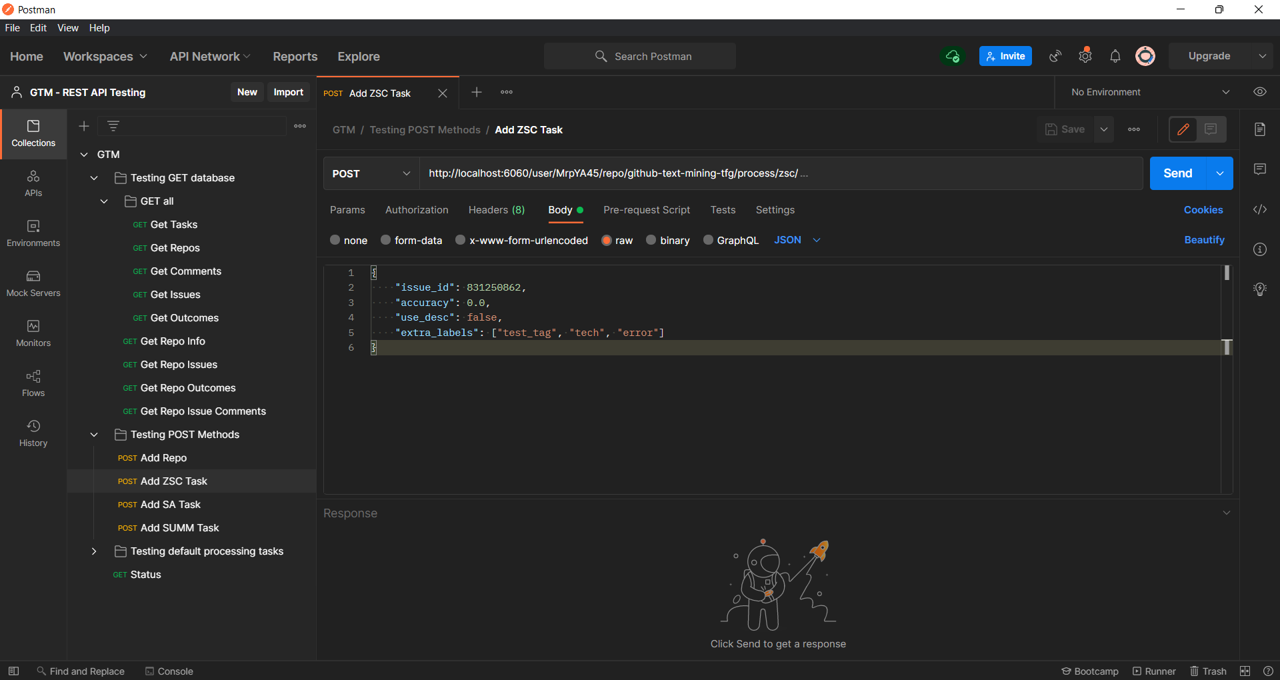
\includegraphics[width=\textwidth]{img/postman_rest_testing.png}
	\caption{Colección de pruebas de comportamiento en Postman.}
	\label{fig:postman_rest_testing}
\end{figure}
\apendice{Documentación de usuario}

\section{Introducción}

La documentación de usuario tiene como finalidad presentar una guía de requisitos necesarios para el correcto funcionamiento de la aplicación, un manual de instalación guiado paso a paso y la presentación de las opciones de interacción disponibles a través de la aplicación web para la obtención de resultados.

\section{Requisitos de usuarios}

Los requisitos de usuario sugieren una serie especificaciones hardware y software del equipo anfitrión de la aplicación de modo que el proyecto cumpla con los requisitos funcionales y no funcionales. Estas características son las siguientes:

\begin{itemize} \setlength\itemsep{0.2em}
    \item Sistema operativo Windows 10 o Ubuntu 20.04 o superior.
    \item 6GB de memoria RAM.
    \item 30GB de espacio libre en disco.
    \item Conexión a Internet estable.
    \item Navegador web: Google Chrome 96, Microsoft Edge 96, o Mozilla Firefox 94 o superior.
\end{itemize}

\section{Instalación}

En el siguiente apartado se presentan las instrucciones a través de las cuales establecer un entorno de desarrollo que disponga del código fuente, utilidades, complementos y ejecutables requeridos para la puesta en marcha del proyecto. 

\subsection{Prerrequisitos}
El código fuente del proyecto se ha implementado haciendo uso de los lenguajes de programación \textbf{Python} y \textbf{JavaScript}. En el caso de Python este se requiere para las implementaciones llevadas a cabo en el apartado del front-end. El uso de JavaScript se debe al desarrollo de la aplicación web, implementada sobre el entorno de ejecución \textbf{NodeJS}. A continuación se incluyen las versiones requeridas por la aplicación para asegurar su correcto funcionamiento:
\begin{itemize}
    \item \textbf{Python 3.9.6} o superior.
    \item \textbf{NodeJS 14.17.4} o superior.
    \item \textbf{Docker 20.10.12} o superior.
    \item \textbf{Docker Compose 1.29.2} o superior.
\end{itemize}

\subsection{Obtención el proyecto}

El proyecto se encuentra alojado en un repositorio de GitHub de acceso libre. Para proceder con la obtención de una copia local de los ficheros se recurrirá a un software de control de versiones que ofrezcan soporte a repositorios de GitHub como \textbf{Git} o \textbf{GitHub Desktop}. También es posible la descarga directa de los ficheros a través de la dirección de GitHub en la cual se encuentra alojado el repositorio. La dirección de acceso al repositorio es la siguiente:

\vspace{0.5cm}
\centerline{\texttt{\url{https://github.com/MrpYA45/github-text-mining-tfg}}}
\vspace{0.4cm}

En caso de que se haya decidido escoger el popular software de control de versiones Git el comando requerido para la obtención de los archivos es el siguiente:

\vspace{0.5cm}
\centerline{\texttt{git clone https://github.com/MrpYA45/github-text-mining-tfg}}
\vspace{0.4cm}

\begin{figure}[!ht]
	\centering
    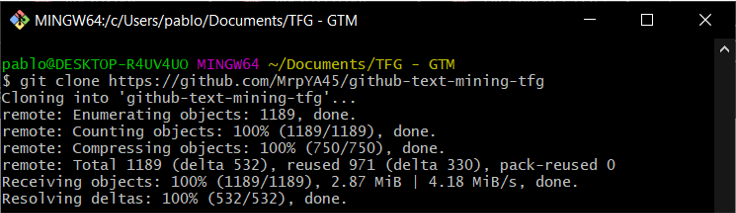
\includegraphics[width=\textwidth]{img/git_gtm.png}
	\caption{Obtención del repositorio mediante Git.}
	\label{fig:git_gtm_mu}
\end{figure}

\subsection{Instalación de las dependencias de la aplicación web}
A continuación, se procederá con la instalación de las dependencias de la aplicación web. Esta se encuentra construida sobre el entorno de ejecución NodeJS basado en JavaScript. La aplicación web también ha sido desarrollada haciendo uso de módulos que simplifican la programación de ciertos aspectos de la web.

Para proceder a la instalación de estas dependencias se deberá situar la terminal en la carpeta \texttt{src/webapp}. El fichero \texttt{package.json} es el encargado de almacenar el listado con las dependencias necesarias para poder proceder con la instalación, así como los \textit{scripts} que permiten lanzar la aplicación. Para proceder con la instalación de los ficheros necesarios se deberá recurrir al siguiente comando:

\vspace{0.5cm}
\centerline{\textbf{Windows/MacOS/Linux: } \texttt{npm install}}
\vspace{0.4cm}

\subsection{Lanzamiento de los servicios del back-end}

El lanzamiento de los servicios del back-end se realizará por medio del uso de las herramientas \textbf{Docker} y \textbf{Docker Compose}, para las cuales se ha diseñado una configuración que permite mantener cada uno de los servicios y la base de datos en contenedores independientes.

El primer paso consistirá en la obtención de las imágenes que se ejecutarán en el interior de los contenedores. Para ello, situándonos en la directorio raíz del proyecto, se deberá ejecutar el comando de construcción que se incluye a continuación. Se ha de tener en cuenta que la primera ejecución del comando requiere de la descarga de numerosos archivos pesados, por ello por lo que el proceso puede alargarse durante varios minutos.

\vspace{0.5cm}
\centerline{\textbf{Windows/MacOS/Linux:}}
\centerline{\texttt{docker-compose -f docker/config/docker-compose.yml build}}
\vspace{0.4cm}

Una vez se ha completado el proceso de generación de las imágenes se deberá proseguir con el levantamiento de los contenedores que contendrán dichas imágenes. En una primera instancia este proceso requiere de un extenso tiempo de espera durante el cual se procede a la descarga e instalación de las dependencias requeridas por los servicios en el interior de los propios contenedores.

\vspace{0.5cm}
\centerline{\textbf{Windows/MacOS/Linux:}}
\centerline{\texttt{docker-compose -f docker/config/docker-compose.yml up}}
\vspace{0.4cm}

El servicio con un mayor tiempo de despliegue inicial resulta ser el servicio de procesamiento denominado \textit{gtmprocessing}, el cual puede llegar a requerir de entre 10 y 15 minutos en su arranque. Ante la pobre vivacidad que se presenta en el proceso de obtención de los modelos se recomienda realizar comprobaciones periódicas a través del siguiente comando.

\vspace{0.5cm}
\centerline{\textbf{Windows/MacOS/Linux: } \texttt{docker logs gtmprocessing -t}}
\vspace{0.4cm}

Esta orden permite obtener un visualizar la actividad que se está produciendo en el interior del contenedor. A través de esta salida se podrá comprobar el estado de la descarga de los modelos.

\subsubsection{Configuración inicial de los servicios}

Una vez finalizado el proceso de configuración inicial se deberá verificar que se han generado correctamente los ficheros de configuración. Estos ficheros se encuentran en el interior de cada uno de los servicios en la ruta \texttt{/src/backend/\%service\_name\%/config}.

Verificada la existencia de estos ficheros se deberán detener los contenedores para poder proceder a su pertinente configuración.

\vspace{0.5cm}
\centerline{\textbf{Windows/MacOS/Linux:}}
\centerline{\texttt{docker-compose -f docker/config/docker-compose.yml stop}}
\vspace{0.4cm}

Cada servicio dispone de una carpeta \textit{gtmcore} en su configuración que permite alterar los parámetros de conexión con la base de datos. Por defecto, estos ficheros se generan con una configuración básica de acuerdo con la configuración de la base de datos establecida en el fichero de variables de entorno de Docker localizado en la siguiente ruta \texttt{docker/services/.env}. Se recomienda encarecidamente modificar estos valores en caso de lanzar la aplicación en algún entorno de producción.

Finalmente, el servicio de extracción dispone de una segunda carpeta de configuración denominada \textit{gtmprocessing}. En su interior se encuentra un fichero de configuración que se requiere completar para lograr la extracción de la información de los repositorios. Este fichero solicita un token de acceso personal de GitHub.

Una vez se haya completado la configuración de los servicios se deberá volver a levantar los contenedores con el comando señalado anteriormente. En el momento en que los servicios se encuentren completamente desplegados será posible acceder a la API REST de la aplicación por medio de consultas a la dirección \url{http://localhost:6060/}.

\subsubsection{Obtención de un token de acceso personal de GitHub}

La obtención de un token de acceso personal de GitHub requiere de encontrarnos registrados en la plataforma. Una vez en ella se puede solicitar el token desde el apartado de \textit{Settings}, \textit{Developer Settings}, y seleccionar el apartado \href{https://github.com/settings/tokens}{\textit{Personal Access Tokens}}.

La generación de un token requiere del establecimiento de un periodo de caducidad y de la selección de una serie de permisos básicos para poder realizar ciertas acciones. El uso básico de las peticiones que se realizan por parte de la aplicación implica que solo se requiere del permiso de acceso a repositorios públicos (véase \autoref{fig:gen_github_access_tokens_mu}).

\begin{figure}[!ht]
	\centering
    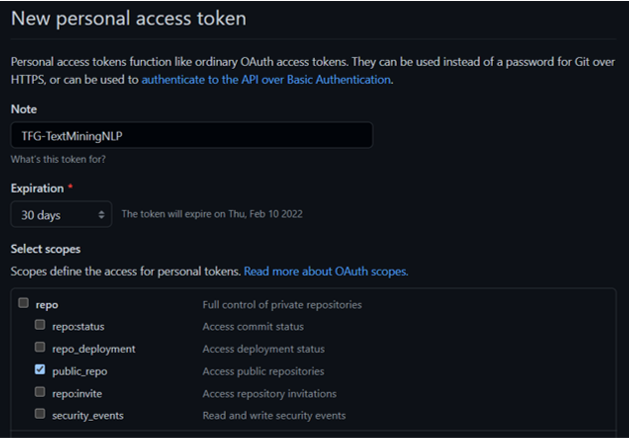
\includegraphics[width=\textwidth]{img/gen_github_access_tokens.png}
	\caption{Generación del Token de Acceso Personal en GitHub.}
	\label{fig:gen_github_access_tokens_mu}
\end{figure}

\subsection{Lanzamiento de la aplicación web mediante NodeJS}

El lanzamiento de aplicación web solamente requiere de la situación de la terminal en la ruta donde se localiza los ficheros de la aplicación web (\texttt{src/webapp}) y la introducción del siguiente comando. 

\vspace{0.5cm}
\centerline{\textbf{Windows/MacOS/Linux: } \texttt{npm start gtm-webapp}}
\vspace{0.4cm}

Tras su ejecución se producirá el despliegue de la aplicación en un servidor de NodeJS y la apertura automática de una ventana en el navegador web presentando al usuario la web. En caso de que esto no suceda por algún motivo desconocido, la aplicación web se encuentra accesible desde la siguiente dirección \url{http://localhost:3000/}.

\section{Manual del usuario}

El manual de usuario tiene como finalidad ilustrar el uso de la interfaz web de la aplicación.

\subsection{Selección y obtención de repositorios}

El primer paso requerido para explotar las funcionalidades de la aplicación consiste en incorporar los datos de los repositorios a la aplicación. Para ello, el usuario deberá hacer clic sobre el apartado ''\textbf{Repositorios}'' de la web. En esta sección se podrá observar un listado de los repositorios disponibles debido a que hayan sido cargados previamente por el usuario, así como un formulario en una sección inferior que permite incorporar nuevos repositorios al sistema (véase \autoref{fig:webapp_list_and_get_repo}).

\begin{figure}[!ht]
	\centering
    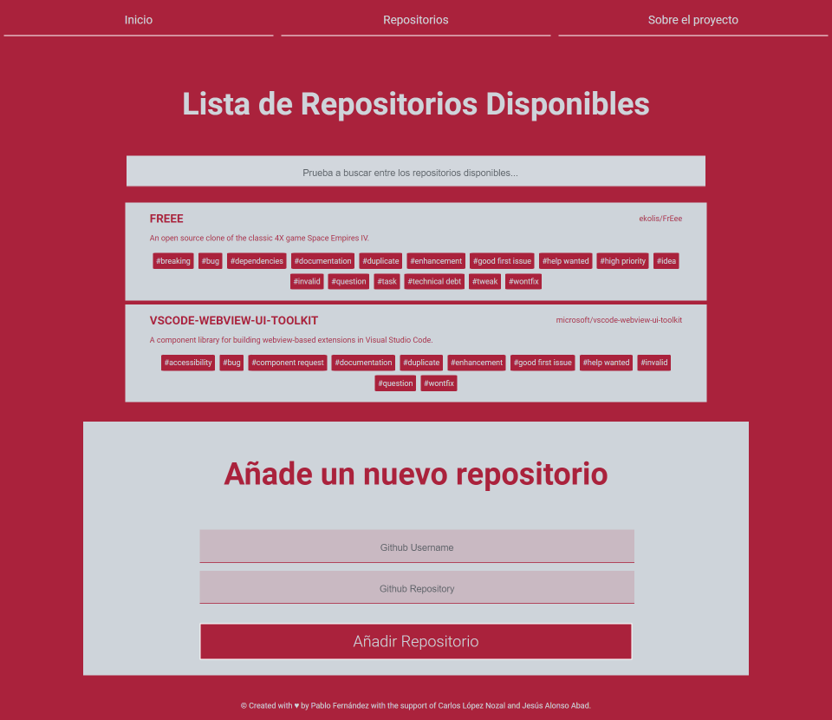
\includegraphics[width=\textwidth]{img/webapp_list_and_get_repo.png}
	\caption{Sección ''\textbf{Repositorios}'' de la aplicación web.}
	\label{fig:webapp_list_and_get_repo}
\end{figure}

El procedimiento para incorporar nuevos repositorios requiere de la introducción de una combinación válida de usuario y repositorio de \textbf{GitHub}. Una vez se introduzcan los datos y se pulse sobre el botón de añadir repositorio se encolará dicha petición, siempre y cuando el \textit{back-end} de la aplicación se encuentre debidamente desplegado. El usuario recibirá una notificación indicando si la petición ha podido ser encolada satisfactoriamente o no.

Tenga en cuenta que la introducción de una combinación incorrecta no producirá un error debido a que la notificación solo indica la recepción del trabajo por parte del \textit{back-end}, no su resultado. En caso de que esta combinación resulte incorrecta la tarea quedará rechazada por el \textit{backend} y el proceso no continuará.

Una vez completado el formulario el usuario será redirigido a una nueva pestaña mientras se produce la extracción de los datos. En caso de que se le notifique que el proceso no ha podido continuar, regrese a la pestaña anterior. La detección de una combinación incorrecta no dispone de indicativos visuales, si detecta largos tiempos de espera incoherentes con el tamaño de su repositorio (calculado en función del número de incidencias y sus comentarios), por favor regrese a la sección de Repositorios.

\subsection{Lanzar experimentos}

Una vez la descarga de la información del repositorio se haya completado satisfactoriamente el usuario deberá ser capaz de poder visualizar a una nueva sección de la aplicación. Esta vista presenta una introducción con los datos principales del repositorio y una serie de formularios de acuerdo con los experimentos disponibles.

\subsubsection{Zero-Shot Classification}

Este formulario permite al usuario la aplicación de un modelo de clasificación Zero-Shot sobre las incidencias del repositorio (véase \autoref{fig:webapp_zsc_form}). El objetivo de este experimento consiste en, partiendo de una incidencia y de una serie de etiquetas, asignar una puntuación entre 0 y 1 a cada etiqueta de acuerdo con la probabilidad de que su temática se corresponda con la temática de la incidencia. Por defecto, las únicas etiquetas utilizadas son aquellas definidas por el repositorio para su clasificación manual.

\begin{figure}[!ht]
	\centering
    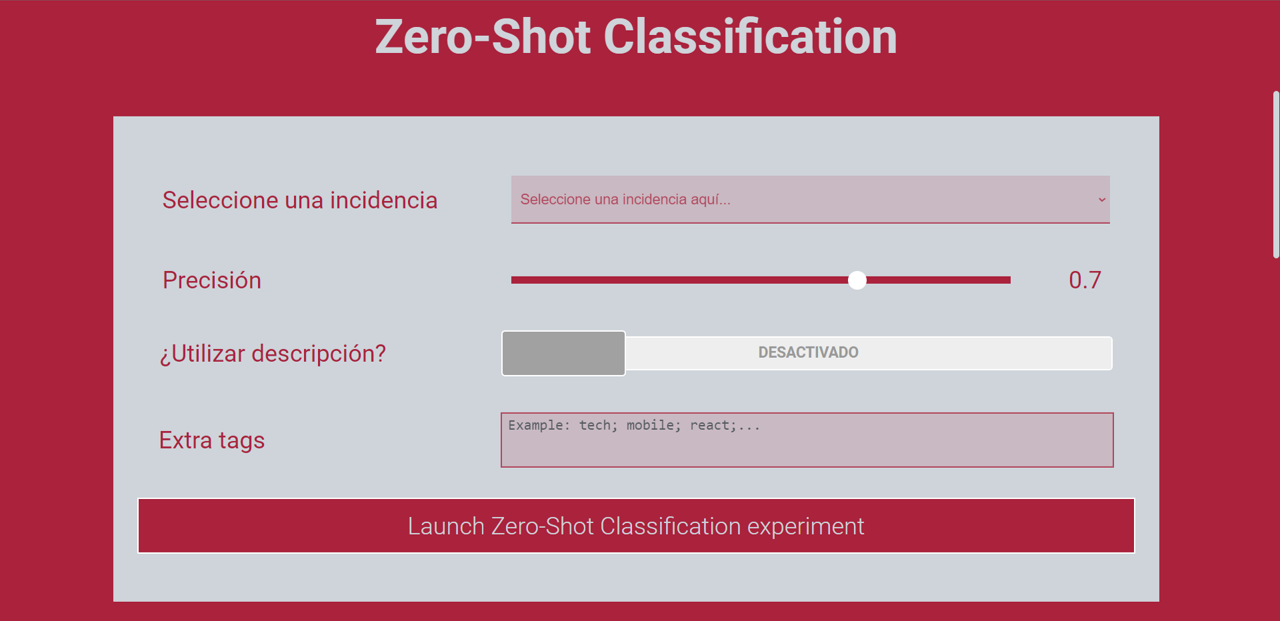
\includegraphics[width=\textwidth]{img/webapp_zsc_form.png}
	\caption{Formulario de lanzamiento de experimento de Zero-Shot Classification.}
	\label{fig:webapp_zsc_form}
\end{figure}

Los parámetros disponibles son los siguientes: 

\begin{itemize} \setlength\itemsep{0.2em}
    \item \textbf{Selección de incidencia}. Este parámetro permite seleccionar mediante un desplegable las incidencias del repositorio de acuerdo con su título. Es posible que observe más incidencias que las disponibles en su sección homónima en su repositorio de GitHub. Esto se debe a que GitHub trata internamente las ''\textit{pull request}'', o solicitudes de incorporación de cambios, como una extensión vitaminada de las incidencias. Como estas también incluyen un apartado de discusión, también es posible trabajar con ellas durante los experimentos.
    \item \textbf{Precisión}. El \textit{slider} de la precisión permite al usuario indicar un umbral a partir del cual las etiquetas que se encuentren por debajo de este no serán mostradas como resultado válido.
    \item \textbf{Utilizar descripción}. Este parámetro permite otorgar un mayor contexto al modelo incluyendo la información correspondiente con la descripción de la incidencia en la realización de sus operaciones. Por defecto el modelo sólo utiliza la información deducida a partir de su título.
    \item \textbf{Etiquetas extra}. Este parámetro permite añadir etiquetas fuera de aquellas declaradas por el propio repositorio en GitHub. Las etiquetas deberán introducirse en el cuadro de texto separadas haciendo uso del carácter punto y coma entre ellas.
\end{itemize}

Los resultados del experimento se presentan en forma de de un gráfico circular que contiene aquellas etiquetas que sobrepasan el umbral establecido en los parámetros. El tamaño de las secciones representa la probabilidad de pertenencia a cada una de las temáticas propuestas (véase \autoref{fig:webapp_zsc_output}).

\begin{figure}[!ht]
	\centering
    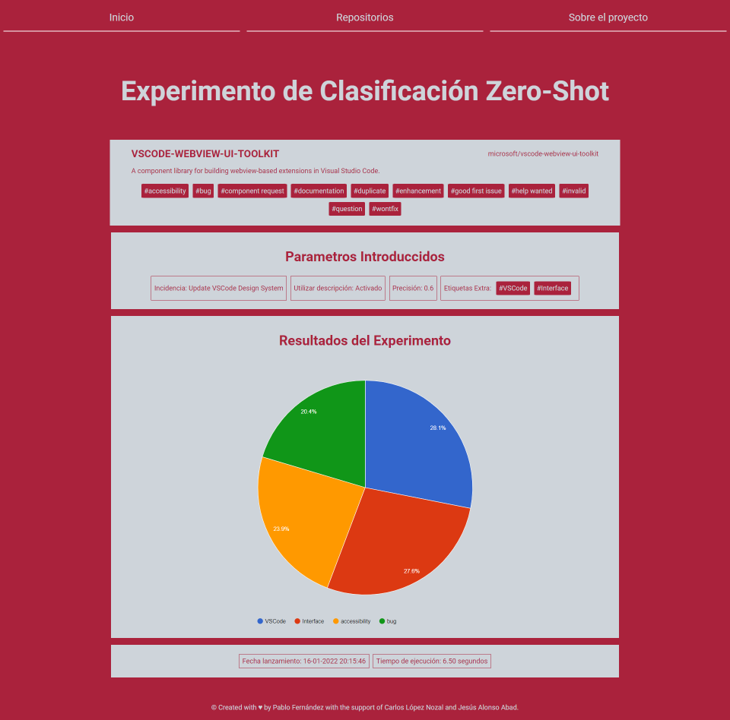
\includegraphics[width=\textwidth]{img/webapp_zsc_output.png}
	\caption{Resultados obtenidos en un experimento de Zero-Shot Classification.}
	\label{fig:webapp_zsc_output}
\end{figure}

\subsubsection{Sentiment Analysis}

Este formulario permite al usuario la aplicación de un modelo de análisis de sentimientos sobre las incidencias del repositorio (véase \autoref{fig:webapp_sa_form}). La finalidad de este experimento radica en la obtención de una puntuación que defina la actitud de los usuarios participantes en la discusión generada por una incidencia. La puntuación obtenida se calcula por cada fragmento y puede variar entre 0 y 1, siendo cero la representación de una expresión de sentimientos muy negativos, y uno la representación de una expresión de sentimientos muy positivos. 

\begin{figure}[!ht]
	\centering
    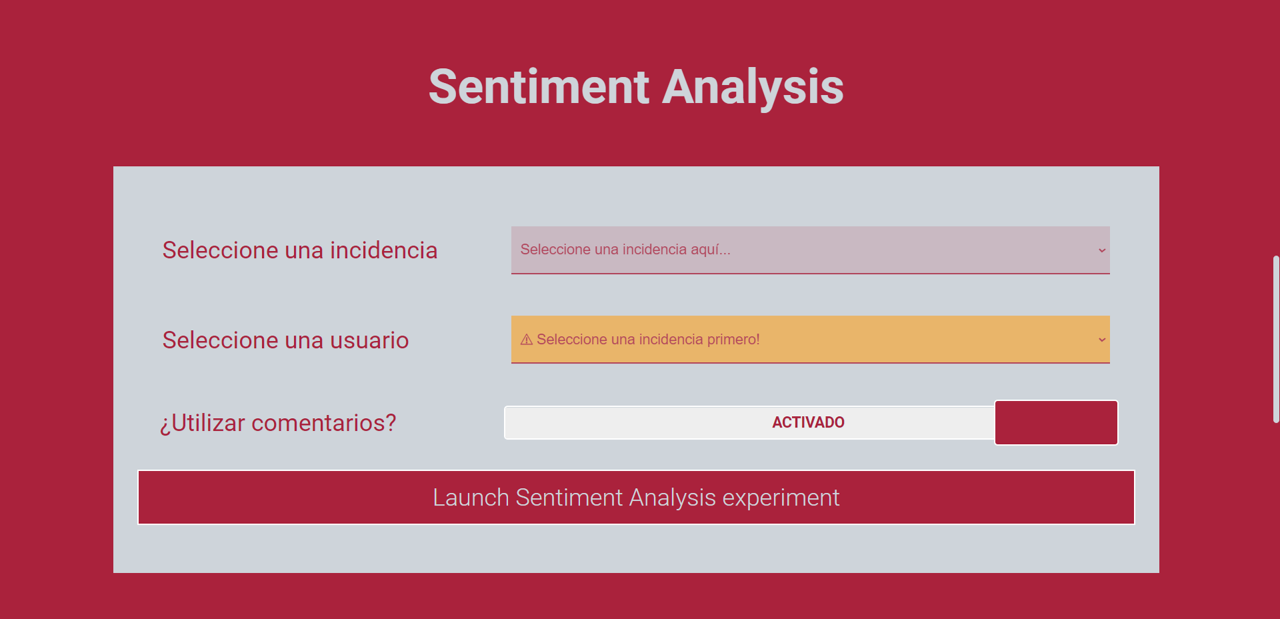
\includegraphics[width=\textwidth]{img/webapp_sa_form.png}
	\caption{Formulario de lanzamiento de experimento de Sentiment Analysis.}
	\label{fig:webapp_sa_form}
\end{figure}

Los parámetros disponibles son los siguientes:

\begin{itemize} \setlength\itemsep{0.2em}
    \item \textbf{Selección de incidencia}. Este parámetro permite seleccionar mediante un desplegable las incidencias del repositorio de acuerdo con su título. 
    \item \textbf{Selección de usuario}. Este parámetro permite filtrar los comentarios de la incidencia que van a ser tomados como entrada del modelo a aquellos realizados exclusivamente por dicho usuario.
    \item Utilizar comentarios. Este parámetro tiene como finalidad permitir la realización del análisis de sentimientos de la entrada inicial de la incidencia, excluyendo sus comentarios tanto del autor como del resto de participantes en la conversación.
\end{itemize}

Los resultados del experimento se presentan haciendo uso de un gráfico de barras verticales. Cada barra azul representa la puntuación otorgada a un comentario, siendo la línea horizontal roja el indicador de la puntuación media obtenida de acuerdo con los parámetros introducidos (véase \autoref{fig:webapp_sa_output}).

\begin{figure}[!ht]
	\centering
    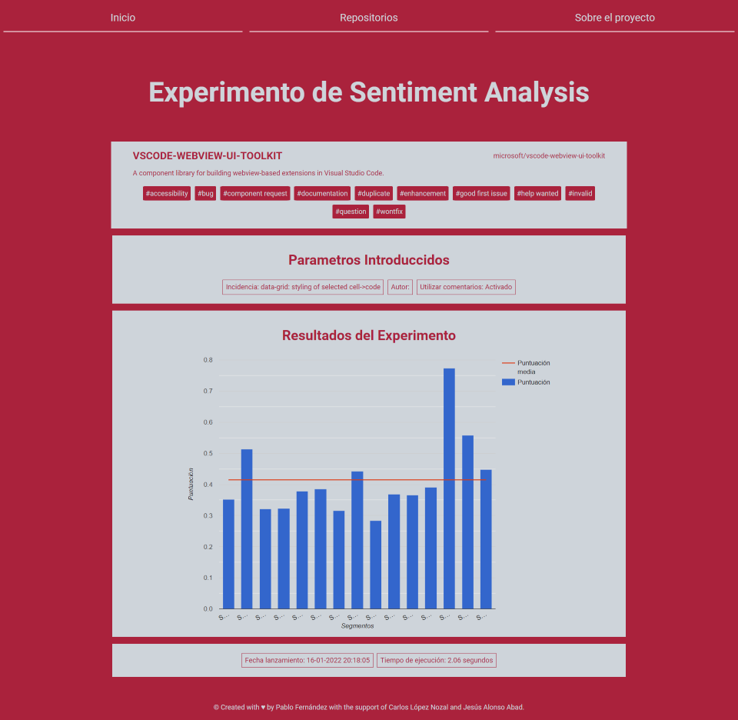
\includegraphics[width=\textwidth]{img/webapp_sa_output.png}
	\caption{Resultados obtenidos en un experimento de Sentiment Analysis.}
	\label{fig:webapp_sa_output}
\end{figure}

\subsubsection{Summarization}

Este formulario permite al usuario el lanzamiento de un experimento de generación de resúmenes abstractivos sobre las incidencias del repositorio (véase \autoref{fig:webapp_summ_form}). La finalidad de este experimento consiste en generar un fragmento de texto que resuma el contenido tratado por la incidencia. El modelo se aplica de manera individual a cada comentario y posteriormente se procede a la concatenación de los resultados para obtener un resumen general del tema tratado en la discusión de la incidencia. Este experimento cuenta con limitaciones lingüísticas debido a que el modelo utilizado que solo ofrece soporte a textos escritos en inglés.

Los parámetros disponibles son los siguientes:

\begin{figure}[!ht]
	\centering
    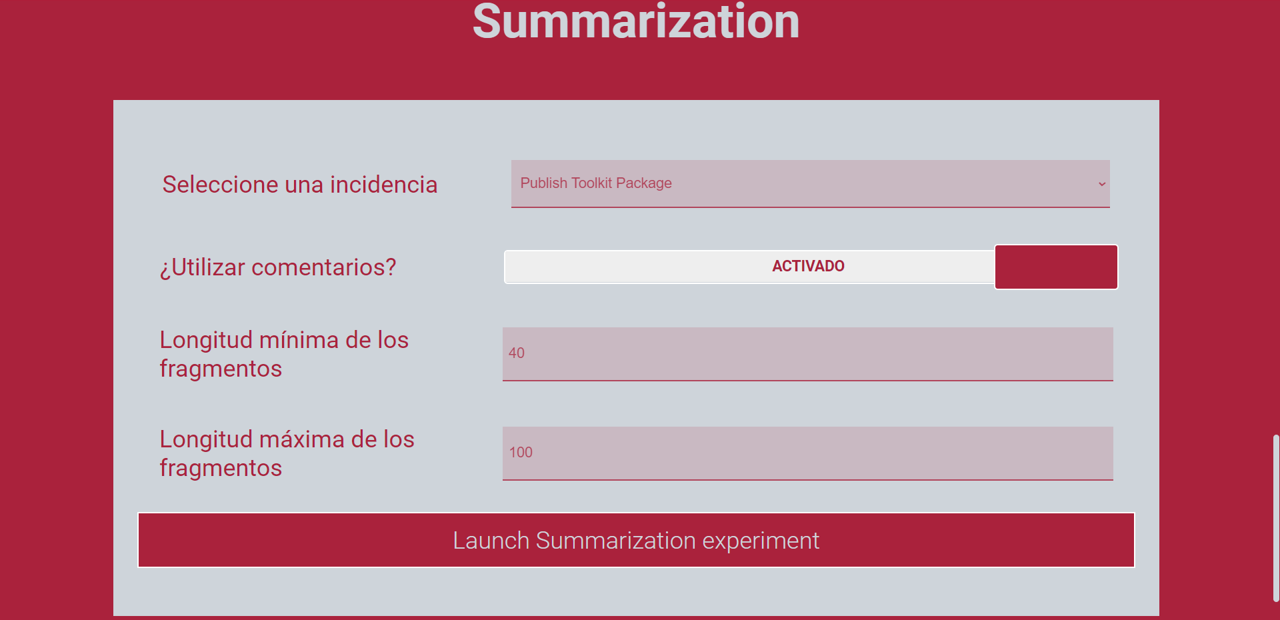
\includegraphics[width=\textwidth]{img/webapp_summ_form.png}
	\caption{Formulario de lanzamiento de experimento de Summarization.}
	\label{fig:webapp_summ_form}
\end{figure}

\begin{itemize} \setlength\itemsep{0.2em}
    \item \textbf{Selección de incidencia}. Este parámetro permite seleccionar mediante un desplegable las incidencias del repositorio de acuerdo con su título.
    \item \textbf{Utilizar descripción}. Este parámetro permite otorgar un mayor contexto al modelo incluyendo la información correspondiente con la descripción de la incidencia en la realización de sus operaciones. Por defecto el modelo sólo utiliza la información deducida a partir de su título.
    \item \textbf{Longitud mínima de los fragmentos}. Este parámetro permite establecer una longitud mínima de los resúmenes parciales que compondrán el resumen final. Es importante destacar el aspecto de los fragmentos, ya que los fragmentos de las entradas se introducen en el modelo de forma individual, por lo tanto el resumen final se elabora a partir de su concatenación. También se ha de destacar que esta longitud no se corresponde directamente con el número de caracteres debido a las consideraciones tomadas por el \textit{tokenizador} utilizado por los modelos.
    \item \textbf{Longitud máxima de los fragmentos}. Este parámetro permite establecer una longitud máxima de los resúmenes parciales que compondrán el resumen final.
\end{itemize}

Los resultados del experimento proveen al usuario del resumen generado en función del contenido de la incidencia y los parámetros de longitud establecidos para cada fragmento (véase \autoref{fig:webapp_summ_output}).

\begin{figure}[!ht]
	\centering
    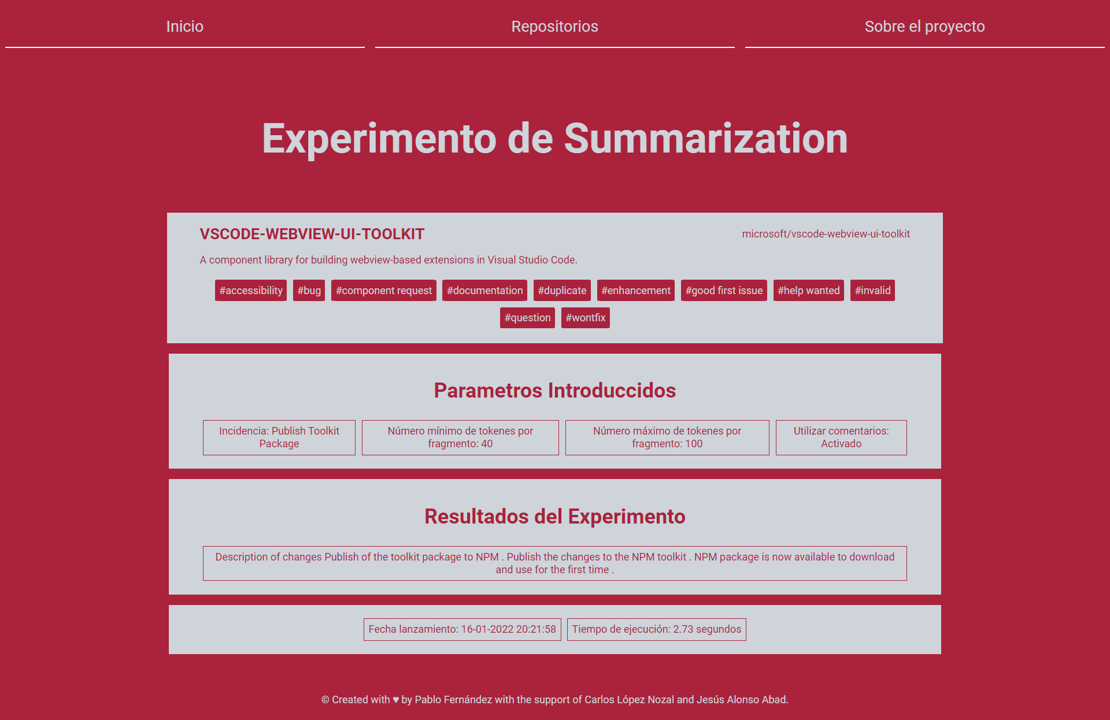
\includegraphics[width=\textwidth]{img/webapp_summ_output.png}
	\caption{Resultados obtenidos en un experimento de Summarization.}
	\label{fig:webapp_summ_output}
\end{figure}


%Where the bibliography will be printed
  \printbibliography

\end{document}
